
\chapter{Light Field Photography}

The propagation of the light rays in the 3D space can be completely described by a 7D continuous function $R(\theta,\phi,\lambda,\tau,V_x,V_y,V_z)$, where $(V_x,V_y,V_z)$ is a location in the 3D space, $(\theta,\phi)$ are propagation angles, $\lambda$ is the wavelength and $\tau$ the time; this function is known as the plenoptic function and describes the amount of light flowing in every direction through every point in space an any time, the magnitude of $R$ is known as the radiance.  In an 1846 lecture entitled "Thoughts on Ray Vibrations" Michael Faraday proposed for the first time that light could be interpreted as a field, inspired by his work on magnetic fields; but the idea of a plenoptic function representing the spectral radiance distribution of rays was first proposed by Adelson and Bergen \cite{Adelson-Plenoptic}. 

\bigskip

\begin{figure}[h!]
\centering
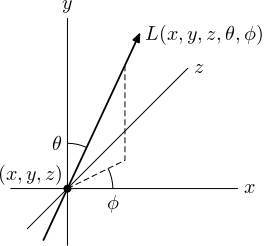
\includegraphics[width=0.5\textwidth]{./Diagrams/Plenoptic_function.jpg}
\caption{Spatio-angular parametrization of the plenoptic function for fixed $\tau$ and $\lambda$. Figure taken from Wikipedia (https://en.wikipedia.org/wiki/Light\_field)}
\end{figure}

\bigskip

In a more practical approach the plenoptic function can be simplified to a 4D version, called 4D Light Field or simply Light Field (abbreviated from now on as LF), denoted as the function $L_4$. The LF quantifies the intensity of static and monochromatic light rays propagating in half space, though this seems like an important reduction of information, this constraint does not substantially limit us in the accurate 3D description of the scene from where the light rays come from.

\bigskip 

 There exists three tipical forms of this 4D approximation: 
\begin{enumerate}
\item The LF rays positions are indexed by their Cartesian coordinates on two parallel planes, also called the two-plane parametrization $L_4(u,v,s,t)$.
\item The LF rays positions are indexed by their Cartesian coordinates on a plane and the directional angles leaving each point, $L_4(u,v,\phi,\theta)$.
\item Pairs of points on the surface of a sphere $L_4(\phi_1,\theta_1,\phi_2,\theta_2)$.
\end{enumerate}

\bigskip

\begin{figure}[h!]
\centering
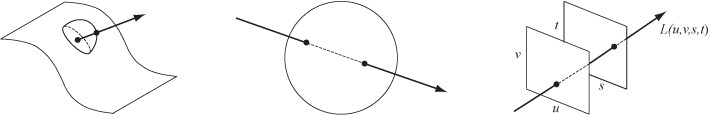
\includegraphics[width=1.0\textwidth]{./Diagrams/Light-field-parametrizations.jpg}
\caption{Three different representations of 4D LF\@. Left: $L_4(u,v,\phi,\theta)$. Center: $L_4(\phi_1,\theta_1,\phi_2,\theta_2)$. Right: $L_4(u,v,s,t)$. Figure taken from Wikipedia (https://en.wikipedia.org/wiki/Light\_field)}
\end{figure}

\bigskip

In this work we will centered our attention in the two plane parametrization $L_4(u,v,s,t)$, if you are interested in the other descriptions we recommend to see \cite{Liang}. In order to understand deeply this way of LF description, lets consider a camera with image plane coordinates $(u,v)$ and the focal distance $f$ moving along the $(s,t)$ plane. 

\bigskip

\begin{figure}[h!]
\centering
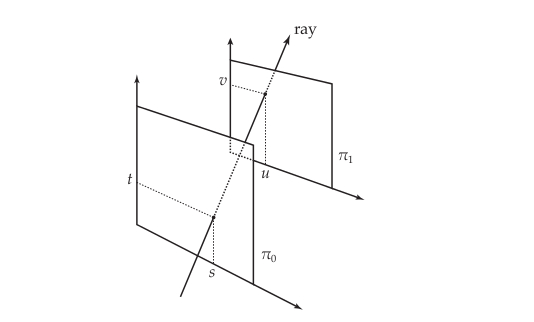
\includegraphics[width=1.0\textwidth]{./Diagrams/two-planes_param.jpg}
\caption{Graphic representation of the two plane parametrization of a single ray on the LF which is parametrized by the intersection $(s,t)$ and $(u,v)$ with planes $\pi_0$ and $\pi_1$, respectively. Figure taken from \cite{Kim-Disney} p.21}
\label{fig:C2S0F3}
\end{figure}

\bigskip

For simplicity one can constrain the vertical camera motion by fixing $s = s_0$ and moving the camera along the $t-axes$ in an straight light motion, in the section~\ref{sec:Epi-geometry} we will see that this constraint leads to an elegant geometric 3D representation of the scene called Epipolar Geometry, this multiview aquisition is refered as parallax only (HPO). Under this constraint, images captured by successive camera positions $t_1$, $t_2$,\ldots\ can be stacked together, and one can also interpret each camera position as a time step.

\bigskip

\begin{figure}[h!]
\centering
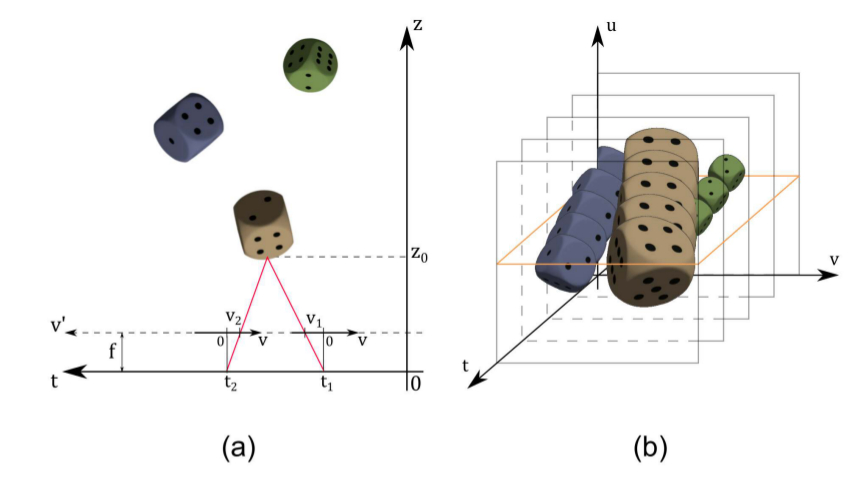
\includegraphics[width= 0.90\textwidth]{./Diagrams/images_stacked.jpg}
\caption{Stacked captured images represented in (b) from the scene setup (a). Figure taken from \cite{LF-Shearlets} p. 2}
\end{figure}

\section{Light Field Photography in the History}

For different reasons of interest for science and art capturing light fields has been an active research area for more than 110 years (the reason will be explained in detail on the section~\ref{sec:LF-applications}). In 1903 Herbert E. Ives \cite{Ives} was the first to realize that the light field inside a camera can be recorded by placing a pinhole or lenslet arrays in front of a film sensor (what is know as pinhole camera). On the other hand, in 1908 the french physicist and Nobel laureate Gabriel Lippmann published two articles about something that he called \textit{photographie int\'egrale} (translated as integral photography) \cite{Lippmann} in which he describes an imaging apparatus with an arrange of small lenses on a 2D grid that are able to capture multiple images of a scene with viewpoint variations; the captured scene is reproduced in 3D as the viewer sees the parallax while the viewpoint changes. Is quite surprising that almost 110 year ago he could have the idea that modern state of the art LF aquisition systems use nowadays. 

\bigskip

Even some experiments to aquire the Light Field of a static scene were already proposed since the beginning of the XX century, the first contribution on the mathematical formalization of the Light Field Theory were proposed in 1991, when Adelson and Bergen \cite{AdelsonBergen} found a way to systematically categorize the visual elements in \textit{early vision}, which in combination, form visual information in the world. Here by \textit{early vision} we mean the processes that are involved in the first steps of the visual cortex, namely, basic segmentation, shape detection, motion analysis between others (for further information about \textit{early vision} \cite{Tomasiearly} is highly recommended); sor this purpose Adelson and Bergen defined the \textit{plenoptic function} which was already discussed at the beginning of this Chapter. 

\bigskip

The history of Light Field Theory can be separated in the three main steps in the study of the Light Field: The acquisition, the processing (which include in the most of the cases a geometry proxy) and the rendering, which are closely related, vary in computational complexity and for which there exist plenty of different approaches; in this thesis we will center our study on the first two steps. 

\bigskip

It is also worth to mention that in the last decade two companies had manufactured Cameras that are able to capture the 4D Light Field, also known as plenoptic cameras; the first was Raytrix founded by the german computer scientists Vhristian Perwass and Lennart Wietzke that released their camera in 2010 mostly focused on industrial application on 3D reconstruction (one can see their paper \cite{Raytrix} for a good reference) rather than general consumers. Later in 2012 the american company Lytro came out with a plenoptic camera that was the first consumer light field camera for the general public, that has as a principal feature the possibility to do refocusing in the pictures taken by the camera (as a reference for this camera we recommend to read the Stanford Technical Report written by the CEO of the company Ren Ng \cite{Lytro}). Both companies produce cameras that capture the light field using an array of lenses, this and other LF acquisition setting will be discuss in the next section.

\bigskip

\begin{figure}[h!]
\centering
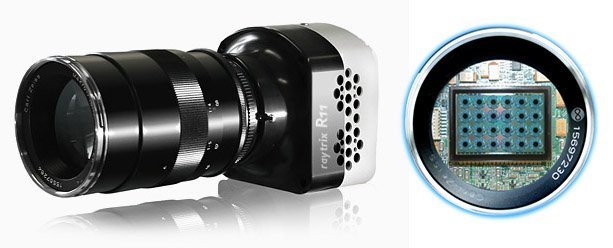
\includegraphics[width= 0.90\textwidth]{./Diagrams/raytrix.jpg}
\caption{Industrial plenoptic camera Raytrix R11, produced by Raytrix. Figure taken from \url{https://petapixel.com/assets/uploads/2010/09/raytrix.jpg}}
\end{figure}

\bigskip

\begin{figure}[h!]
\centering
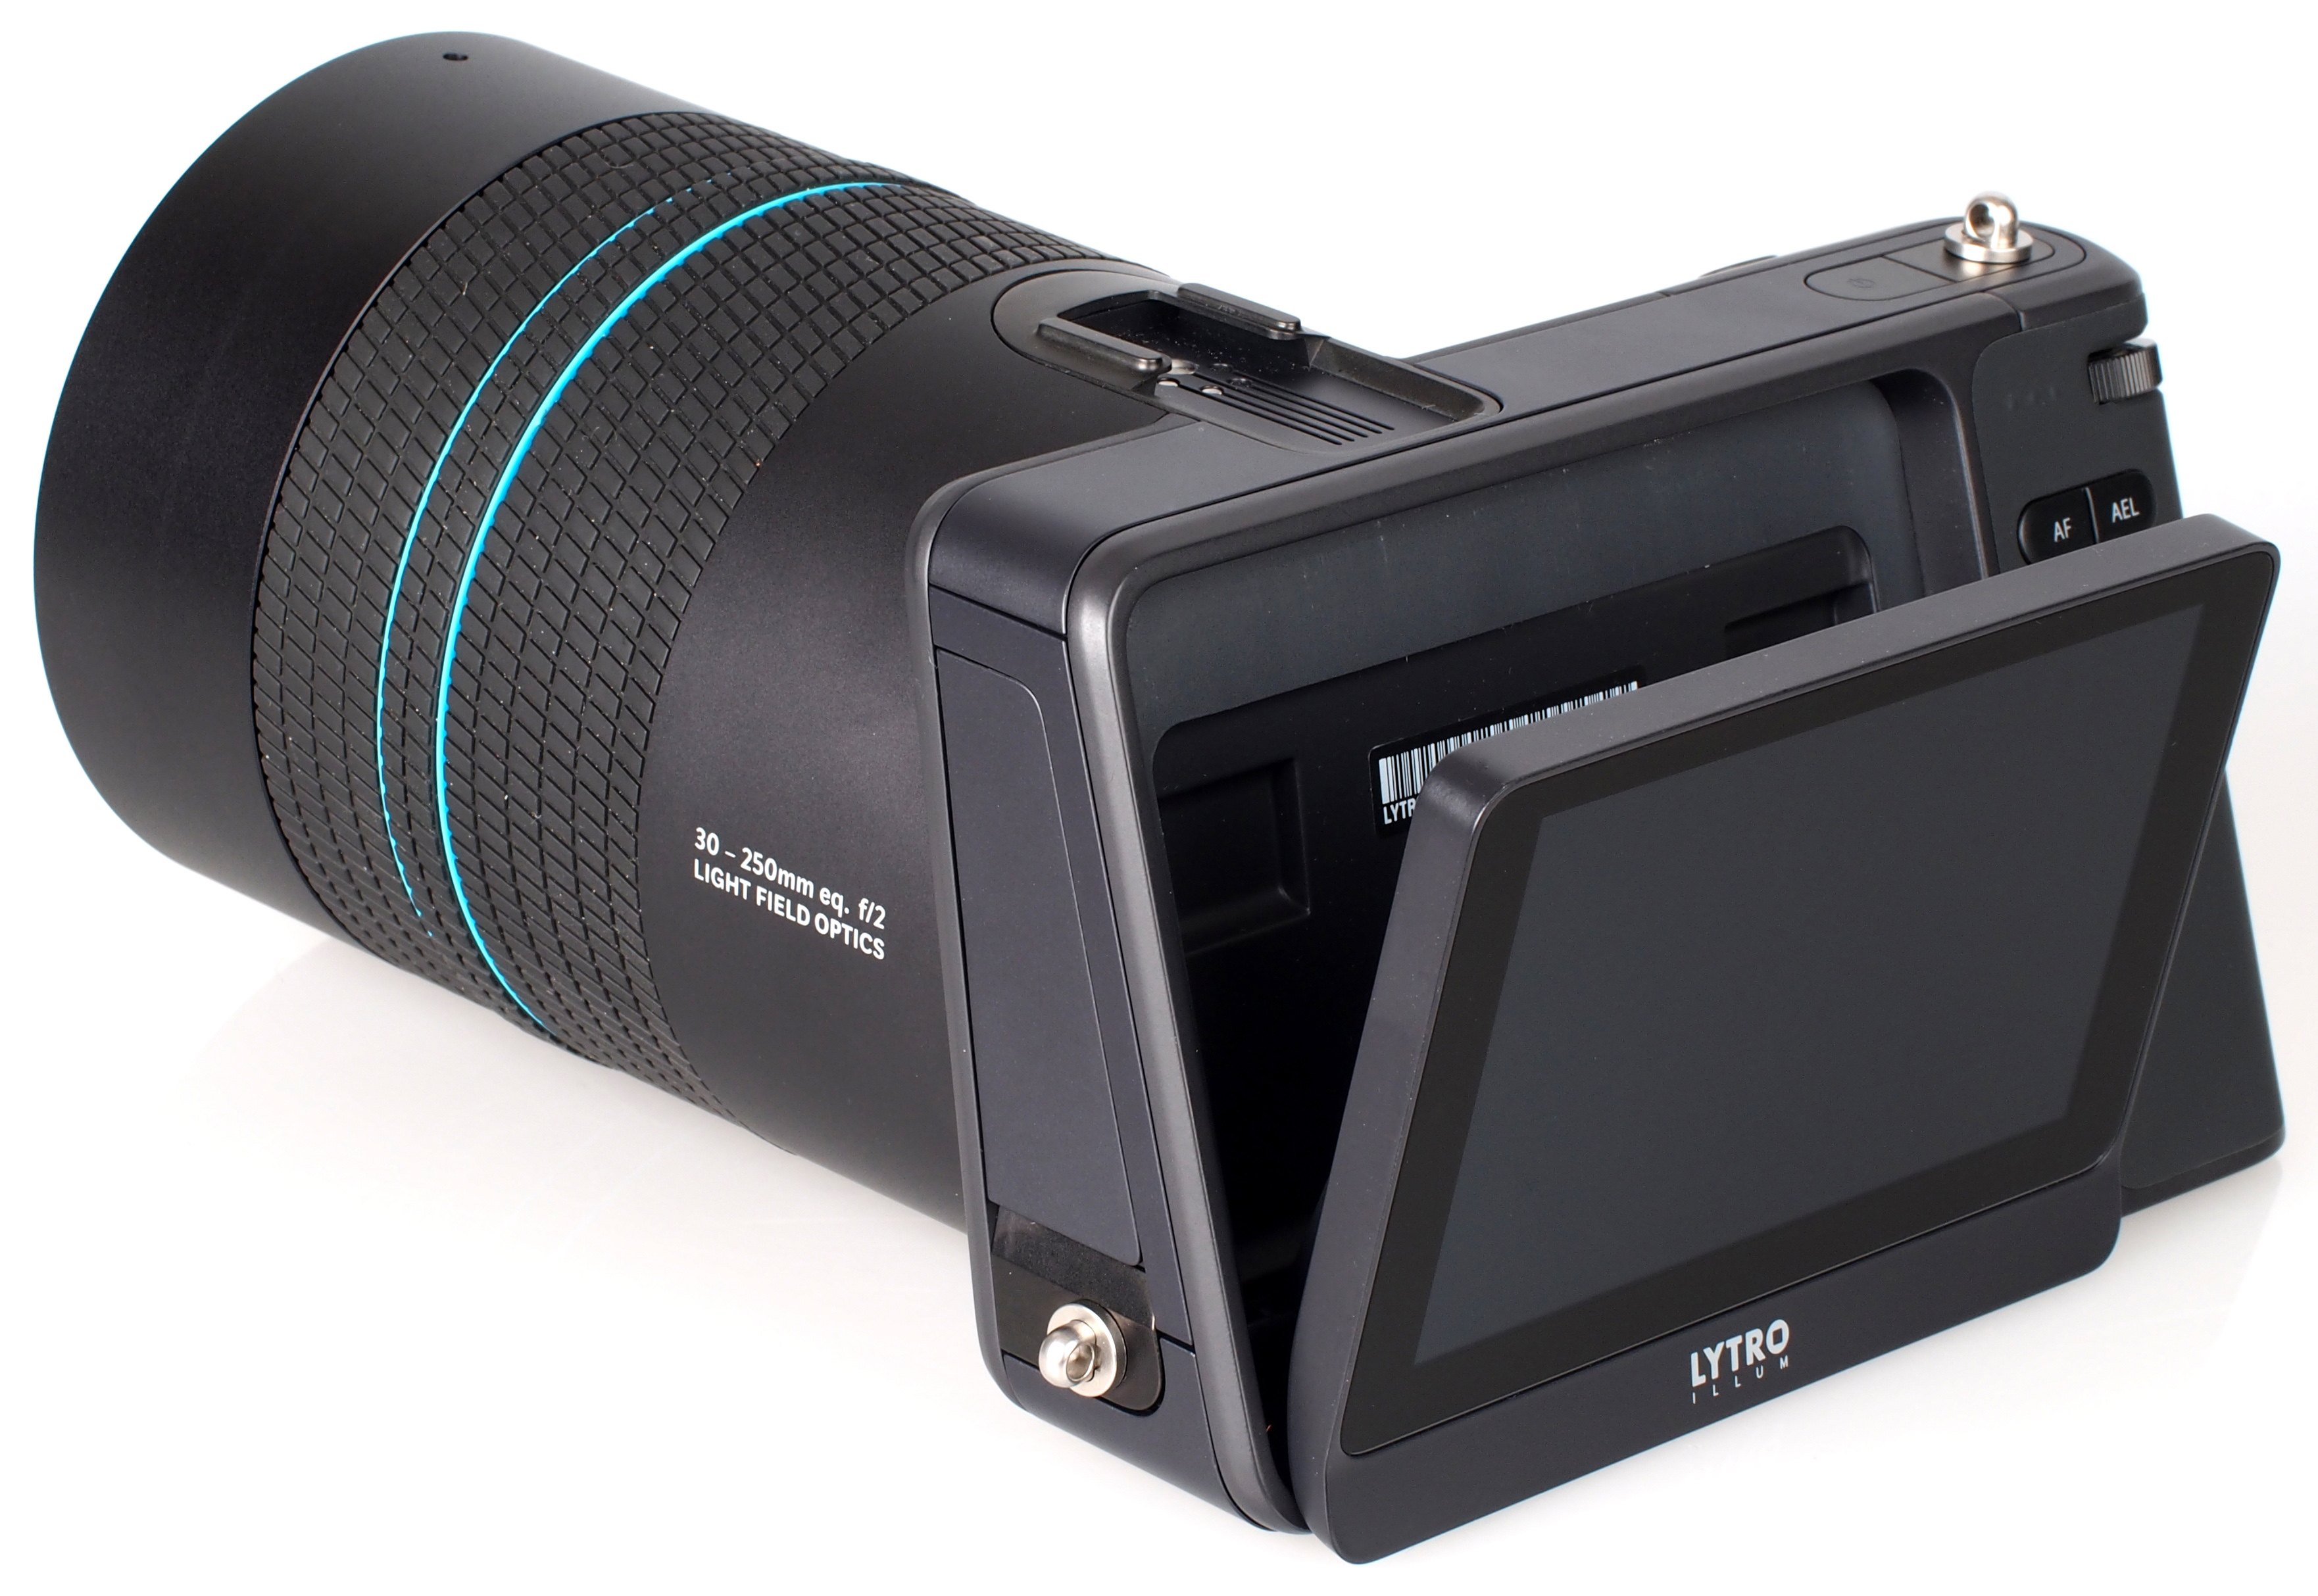
\includegraphics[width= 0.70\textwidth]{./Diagrams/lytro.jpg}
\caption{Consumer plenoptica camera Lytro Illum, produced by Lytro. Figure taken from \url{https://www.ephotozine.com/articles/lytro-illum-review-26434/images/highres-Lytro-Illum-6_1414410926.jpg}}
\end{figure}

\section{Light Field Acquisition Settings}
\label{sec:LF-acquisition}

The first creativity step in the experimental study of Light Field is the form of acquisition; using only our physical intuition is not trivial to come up with an idea of a system that captures faithfully the Light Field coming from a static scene that will be able to be processed by some straight-forward algorithm. From the beginning of the last century until today, scientists, engineers and hobbyists have proposed different approaches for the Light Field Acquisition Settings. 

\bigskip

As we have seen in the last section, the first attempts of settings were the pinhole camera proposed by Ives and the lenslet array proposed by Lippmann. The next variation of setting was proposed more than eighty years later by Adelson and Wang \cite{AdelsonWang} that in 1992 using the theory of plenoptic function (developed by Adelson itself) presented a design of a plenoptic camera where the light rays that pass through the main lens are recorded sparately using a lenticular array placed on the sensor plane, they used the light field recorded with this camera to obtain the scene depth by analyzing the directional variation of the radiance captured in the image; this is basically the Lippmann design but applied to digital cameras. Ng et al. \cite{Lytro} from Lytro used the same design of Adelson and Wang to produce the Lytro cameras.

\bigskip

\begin{figure}[h!]
\centering
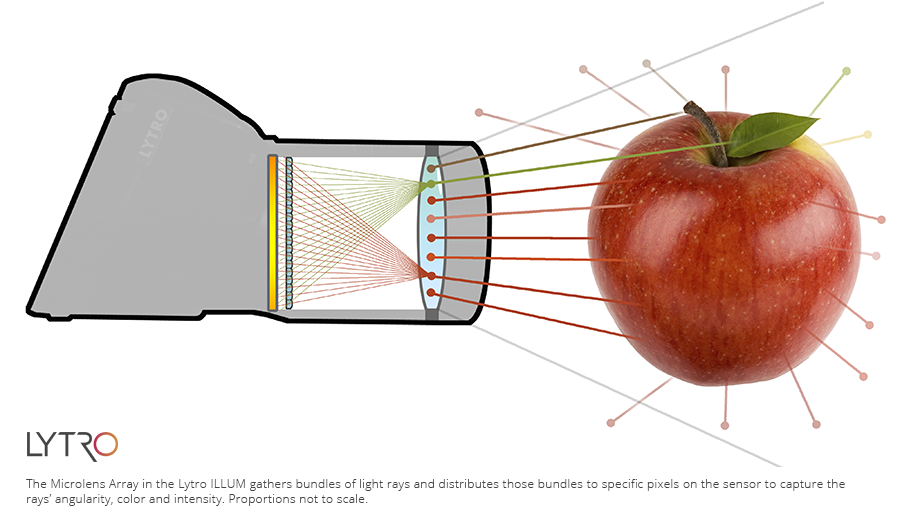
\includegraphics[width= 0.80\textwidth]{./Diagrams/lytro_array.png}
\caption{Diagram of Adelson and Wang design in Lytro cameras. Figure taken from \url{https://s3.amazonaws.com/lytro-corp-assets/blog/Lytro_ILLUM.png}}
\end{figure}

\bigskip

In 2006 Joshi et all \cite{Joshi} used a one-dimensional camera array and a motorized stage for for their real-time matting system. This technique of multicameras/multiviews acquisition is also quite common with camera arrays varying in position and size. The approach followed in this thesis take this technique as acquisition setting, the actual setup used will be explained in more detail in the section~\ref{sec:Sparse-acquisition}. The downside of this acquisition device is that in counterpart of the Lytro camera (hand-held) it can be built without having a priori a designed custom optics, but hey are bulky and often not portable (mechanical tracks are generally quite big and heavy).

\bigskip

A less bulky approach are the ones with Light-modulating codes in mask-based systems, that use coded masks in front of lenses for coded acquisition of the scene. Veeraraghavan et al. \cite{Veeraraghavan} where the first implementing a coded aperture technique to computatinally demultiplex the light rays collected through the camera's main lens. This attempt is less bulky than the multicameras and more light efficient than the pinhole arrays but it sacrifices image resolution, since the number of sensor pixels is the upper limit of the number of light rays captured (problem than camera arrays and lenslets does not have). To overcome this problem, Wetzstein et al. \cite{Wetzstein}, analized multiplexing light fields onto a 2D image sensor and developed a thoery for multiplexing and a computational reconstruction algorithm. 

\bigskip

A significant challenge of acquisition is that the captured set of images is very data-intensive and also redundant, mostly when one tries to recover high resolution light field form images with resolution above $(2000px)^2$. In order to tackle this issue, since the early papers on Light Field, the discussion about compact or sparse representation and compression schemes have played an important role in the area. For instance, Levoy and Hanrahan \cite{Levoy} proposed in 1995 several representations for 4D light fields and apply a lossy vector quantization followed by entropy coding; whereas Gortler et al. \cite{Gortler} in the same year applied standard image compression like JPEG to some of the views and pointed out the importance of depth information for sparser representation.

\bigskip

Later on Wetzstein with the Camera Culture Group of the MIT Media Lab developed a compressive light field camera architecture that allows for higher-resolution light fields to be recovered than previously possible from a single image, using three main components: light field atoms as a sparse representation of natural light fields (that involves dictionary learning which elements are the light field atoms), and optical design that allows for capturing optimized 2D light field projection also based in the coded masks technique, and robust sparse reconstruction methods to recover a 4D ligth field from a single coded 2D projection. In our opinion even this approach allows us to get a very high resolution of light fields, is a trade off by its requirements of high performance computation and its limitations coming from the baised learned dictionaries from a limited set of scenes. 


\bigskip 

\begin{figure}[h!]
\centering
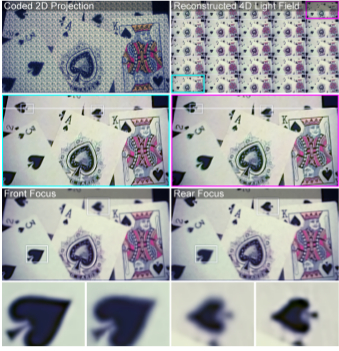
\includegraphics[width= 0.45\textwidth]{./Diagrams/coded-mask.jpg}
\caption{Single coded 2D projection from the work of Wetzstein, Figure taken from \cite{CompressedMIT} p. 8}
\end{figure}


In the multicameras instance, Vargharshakyan et al. \cite{LF-Shearlets} developed in 2015 an image based rendering technique based on light field reconstruction from a limited set of perspective views acquired by cameras, which in that sense is compressed. Even the preprint was presented in 2015, the actual paper was just published this year and it represents a state of the art light field recovery technique. The technique utilizes sparse representation of epipolar-plane images (a very important concept in stereo-vision that will be explained carefully in section~\ref{sec:Epi-geometry}) using as sparsifying system, adapted shearlet transform. This compressive approach was used in this thesis for the light field recovery and we picked it since we consider it as very interesting mathematically since it uses geometry (epipolar-plane representation), compressed sensing (sparse recovery) and functional analysis (shearlet representation). In the next sections and chapters we will cover every detail regarding the technique hoping it is comprehensive for everybody with no expert knowledge of any of the areas but just basic concepts. 


\section{Typical applications for the Light Field Theory}
\label{sec:LF-applications}

We already introduced the concept of 4D Light Field, how this concept has been developed through more than a century already and some techniques of acquisition, but one fundamental question arises; what is the interest of studying Light Fields?, and this question has many answers. Of course the first one is just interest on the mathematical foundation of Early Vision, but this allow us not just to understand more the way the human brain works for vision interpretaton but also to enhance the quality of information of certain spatial scene. For a more clear exposition we will enumarate some of the more remarkable applications of light field recovery:

\begin{itemize}
\item \textbf{Illumination engineering}: With the study of the ligth field one can derive in a closed form the illumination patterns that would be observed on surfaces due to ligth sources of various shapes positioned above these surface. 
\begin{figure}[h!]
\centering
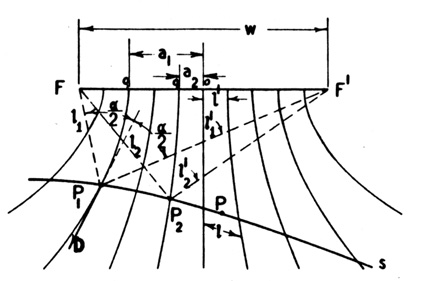
\includegraphics[width= 0.50\textwidth]{./Diagrams/ill_enge.png}
\caption{Downward-facing light source which induces a light field whose irradiance vectors curve otwards, Figure taken from \url{https://en.wikipedia.org/wiki/File:Gershun-light-field-fig24.png}}
\end{figure}

\item \textbf{View synthesis}: One of the most visible applications of the light fields, which centers of the synthesis of intermediate views from a given set of captured views of a 3D visual scene, also called image-based rendering. Immersive visual applications as free viewpoint television and virtual reality require a dense set of images of a scene, but the scene is typically captured by a limited number of cameras that form a coarse set of multiview images. Modern methods for view synthesis are based in two different approaches: estimation of the scene depth and synthesis of novel views based on the estimated depth and the given images, where the depth works as correspondence map for view reprojection (something that could be interpreted as inverse projection). The limitation on this approach is that the quality of depth estimation is dependent on the scene content, causing visually annoying artifacts in the rendered (synthesized) views when the depth map has small deviations (for further information of this one can read \cite{Kim-Zimmer}).

\bigskip

The best approach so far that fixes this problem is based on the concept of plenoptic function and its light field  approximation. The scene capture and intermediate view synthesis problem can be formulated as sampling and consecutive reconstruction (interpolation) of the underlying plenoptic function. LF based methods consider each pixel of the given views as a sample of a multidimensional LF function, thus the unknown views are function values that can be determined after its reconstruction from samples.

\item \textbf{Synthetic aperture photography (Light Field rendering)}: One can approximate the view that would captured by a camera having a finite aperture (non-pinhole) when integrating an appropiate 4D subset of the samples in a light field. This view has a finite depth of field (one can focuse until a finite depth on the scene). One can focus on different fronto-parallel or oblique planes in the scen by shearing the light field before performing this integration (one can check \cite{Isaksen} for the fronto-parallel case). Like in the case of Lytro cameras, this permits its photographs to be refocused after they are taken.

\item \textbf{3D display}: One can present a light field using technology that maps each sample to the appropiate ray in physical space, one obtains then an autostereoscopic visual effect akin to viewing the original scene (hologram-wise). For non digital technologies for doing this one can use holography; digital technologies of 3D display include placing an array of lenslets over a high-resolution display screen, or projecting the imagery onto an array of lenslets using an array of video projectors; if this last one is combined with an array of video cameras, one can capture and display a time-varying light field, which basically constitutes a 3D television system (check \cite{Javidi}).

\item \textbf{Light Field microscopy}: Light field permit manipulation of viewpoint and focus after the imagery has been recorded. By inserting a microlens array into the optical train of a conventional microscope, one can capture light fields of biological specimens in a single photograph. The ability to create focal stacks from a single photograph allows moving or light-sensitive specimens to be recorded, with 3D deconvolution one can produce a set fo cross sections whcih can be cisualized using volume rendering, one very recommended reference on that sense is \cite{Ng-micro}.

\item \textbf{Brain imaging}: Neural activity can be recorded optically by genetically encoding neurons with reversible fluorescent markers that indicate the presence of calcium ions in real time. Since Light field microscopy captures full volume information in a singel frame, it is possible to monitor neural activity in many individual neurons randomly distributed in a large volume at video framerate. A quantitative measurement of neural activity can even be done despite optical aberrations in brain tissue and without reconstructing a volume image \cite{Pegard}.

\item \textbf{Glare reduction}: Glare is a difficulty seeing in the presence of bright light such as direct or reflected light, and arises due to multiple scattering of light inside the camera's body and lens optics and reduces image contrast. While glare has been analyzed in 2D image space, it is useful to identify it as a 4D ray-space phenomenon \cite{Raskar}. By analyzing the ray-space inside a plenoptic camera, one can classify and remove glare artifacts, since in ray-space glare behaves as high frequency noise and can be reduced by outlier rejection (for instance thresholding). This application represents a great solution for some issues in film postproduction.

\end{itemize}

We think this examples of application make very clear the important role that Light Field recovery plays in technology, medicine and art; therefore we also think that is worth to study new optimal methods for this recovery.

\section{Geometric proxy: Stereo Vision and multiview Epipolar Geometry}
\label{sec:Epi-geometry}

3D geometry reconstruction has been an interest of study for decades and there is a plenty of material where one can look at, where many different approaches are presented. One of the first approaches to recover depth information from a dense sequence of images is the seminal work of Bolles et al. \cite{Bolles} a very recommended classic in the topic; though its rendering technique is old and not robust enough for a dense reconstruction of scenes with occlusions, vary illumination and other features; one can use the geometric approach to obtain underlying linear structures of the light field. Due the mathematical simplicity and straight forward implementation of this approach we used this model to approach the Epipolar-plane images of the 3D scene to reconstruct the 4D Light Field, but in this case we have a sparse sequence of images so we used a sparse representation for the epipolar plane to tackle this issue.

\subsection{Epipolar constraint}

One of the fundamental tasks of computer vision is to describe a sscene in terms of coherent threedimensional objects and their spatial relationships. This tasks present clear limitations for two main reasons: 
\begin{itemize}
\item There is an enormous diversity of objects and an almost limitless ways in which they can occur in scenes.
\item Classical images have an inherent ambiguity; since the process of forming an image captures only two of the three dimensions of the scene, an infinity of three-dimensional scenes can give rise to the same two-dimensional image; therefore no single two-dimensional image contains enough information to enable reconstruction of the three-dimensional scen that gave rise to it.
\end{itemize}

Human vision tackles this limitation with the use of knowledge of the scene objects and multiple images, like stereo pairs and image sequences acquired by a moving observer; though the mathematical and computational implementation  of this features is not trivial but using more than one image makes it theoritically possible, under certain circumstances (that go from position of the views to sampling rate) modern techniques on stereo vision have made this possible up to some precision. As we already mention in this thesis we will make use of the epipolar plane image analysis technique.

\bigskip

The epipolar plane image analysis proposed by Bolles \cite{Bolles} is a technique to make a threedimensional description of a static scene from a dense sequence of images; the sequence is dense in the sense that its images form a solid block of data in which the temporal continouity from image to image is equal to the spatial continuity (namely the resolution of the picture). Slices of this block encode the 3D position of objects and occlusion of an object by another.

\begin{figure}[h!]
\centering
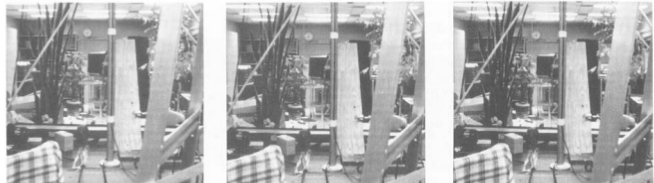
\includegraphics[width= 1\textwidth]{./Diagrams/multi-views1.jpg}
\caption{First three of 125 images taken by Bolles et al. Figure taken from \cite{Bolles} p. 16}
\label{fig:Bollesmultiviews}
\end{figure}

\begin{figure}[h!]
\centering
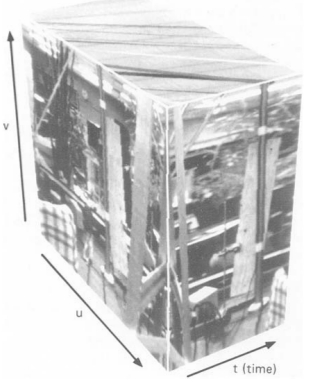
\includegraphics[width= 0.50\textwidth]{./Diagrams/block1.jpg}
\caption{Spatiotemporal solid of data corresponding to the sequence on the Figure~\ref{fig:Bollesmultiviews}, Figure taken from \cite{Bolles} p.16}
\end{figure}


\bigskip

One can supply the separate analysis of both camera motion and object position by an unified treatment of parameters and concentrate solely in object positions, this known motion assumption is appropriate for autonomous vehicles with intertial-guidance systems and some industrial tasks. This assumption is called the \textbf{"epipolar"} constraint and its most important feature is that it reduces the search required to find matching features from two dimensions to one and is derived from the known position of one camera with respect to the other. 

\bigskip

The epipolar constraint as we just mentioned reduces the complexity of matching features between successive images (by search dimensional reduction), even though matching features still one of the most difficult steps in motion processing. In stereo analysis, it is well known that the difficulty of finding matches increases with the distance between the lens centers, so as a second assumption we suppose that the images were taken very close together. 
As another assumption that will simplify the matching of features between seccessive images one assume that the images were taken very close together. 

\bigskip 

At the time that Bolles et al.\ developed the epipolar plane image analysis technique matching features was indeed a very complex task to implement; they did not have digital cameras of high resolution as today, and also the most common algorithms on feature extraction/tracking for motion flow were after 1988 (we will discuss in detail about this on the section~\ref{sec:Sparse-acquisition}) just one year after Bolles proposed this approach. For this reason they developed their own very creative way to track features that is worth to mention shortly, to be able to compare with the modern robust algorithms.  

\subsection{Bolles feature tracking technique and experimental setup}

Bolles and his group in the Artificial Intelligence Center at Menlo Park developed as a feature tracker an edge detection and classification technique for analyzing one slice of the data (spatio-dimensional block of images) at a time. For this end, they adapted this approach to a range sensor, whcih gathered hundreds of slices in sequence. The sensor, a standard structured-light sensor, projected a plane of light onto the objects in the scene and then triangulated the three-dimensional coordinates of points along the intersection of the plane and the objects. The edge detection technique locates discontinuities in one plane and links them to similar discontinuities in previus planes. 

\bigskip

They found out that the spacing between light planes makes a significant difference in the complexity of the procedure that links discontnuities from one plane to the next. When the light planes are close together relative to the size of the object features, matching is essentially easy. When the planes are far apart, the matching is extremely difficult; this effect gives a sampling rate estimate analogous to the Nyquist limit in sampling theory. A deeper sampling analysis will be done in the section~\ref{sec:Sparse-acquisition}. For the physical acquisition of the pictures they borrowed a one-meter-long optical track and gathered multiple images while moving a camera manually along it. 

\bigskip

By different possibilities of camera movements on the track (e.g.\ straight ahead) they realized that it would be easier to make such measurements if they aimed the camera perependicularly to the track instead since the path of a scene point in the multiple views will follow a straight-line trajectory in time (whereas it will follow a hyperbolic trajectory if the camera is moving straight-ahead). 

\begin{figure}[h!]
\centering
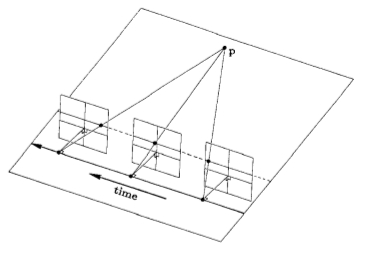
\includegraphics[width= 0.50\textwidth]{./Diagrams/perp-move.jpg}
\caption{Lateral motion with camera perpendicular to the track, Figure taken from \cite{Bolles} p.9}
\end{figure}

The latter can be proven using the next diagram:

\begin{figure}[h!]
\centering
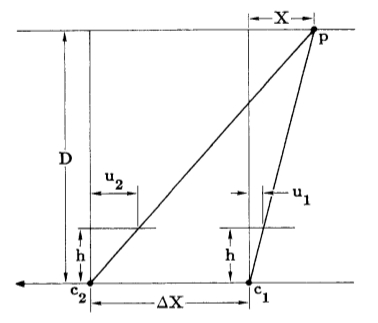
\includegraphics[width= 0.50\textwidth]{./Diagrams/stereo-dist.jpg}
\caption{Lateral motion epipolar geometry, Figure taken from \cite{Bolles} p.9}
\label{fig:LateralMotion}
\end{figure}

Analyzing the figure~\ref{LateralMotion} one can see that the one-dimensional images are at distance $h$ in front of the lens centers, while the feature point $p$ is at a distance $D$ from the linear track along which the camera moves right to left. By similar triangles one has
\begin{equation}
\label{eq:C1S4E1}
\begin{aligned}
\Delta U = u_2-u_1 &= \frac{h(\Delta X+X)}{D}-\frac{hX}{D}\\
                   &= \Delta X\frac{h}{D}
\end{aligned}
\end{equation}
where $\Delta X$ is the distance traveled by the camera along the line, and $\Delta U$ the distance the feature moved in the image plane. By the Equation~\ref{eq:C1S4E1} the change in image position is al inear function of the distnace the camera moves; this equation can be rearranged as follows to yield a simple expression for the distance of a point in terms of the slope of its line in the EPI:

\begin{equation}
\label{eq:C1S4E2}
\begin{aligned}
D = h\frac{\Delta X}{\Delta U}
\end{aligned}
\end{equation}

so if one constructs the spatio-temporal paths of feature points one can get its depth in the scene with respect to the image plane by measuring the slope of its lines with the Equation~\ref{eq:C1S4E2}.

\bigskip

We already mention words as epipolar plane, or epipolar plane image but we have not define anything yet. There are two different approachs to epipolar geometry, one is using functional analysis and permits the study of approximation errors of recovered 4D Light Fields, and the other is geometrical which permits an straight forwart implementation. In this subsection we will shortly expose them. 

\subsection{Functional analysis approach to EPI}

At the beginning of this chapter we mentioned the parallel plane approach to 4D light field (recall Figure~\ref{fig:C2S0F3}), the idea of epipolar geometry is based on this representation. As in Figure~\ref{fig:C2S0F3} lets the two parallel planes be called $\pi_0$ and $\pi_1$ with coordinates $(s,t)$ and $(u,v)$ respectively. In this scheme, the 4D Light Field will be a function $L_4:\mathbb{R}^4\longrightarrow\mathbb{R}^3$ with the radiance $\mathbf{r}\in\mathbb{R}^3$ given as

$$
\mathbf{r}=L_4(u,v,s,t)
$$

If we fix on of the two coordinates on $\pi_0$, say $t$, so that $\pi_0$ reduces to a line, the ray space of the resulting light field will span the $u,v$ and $s$ dimensions of the original ray space; lets called this parameterized light field a 3D light field, and can be denoted as a function $L_3:\mathbb{R}^3\longrightarrow\mathbb{R}^3$. The radiance $\mathbf{r}\in\mathbb{R}^3$ of a light ray is given then as

$$
\mathbf{r}=L_3(u,v,s)
$$

where $s$ is the 1D ray origin and $(u,v)$ represent the 2D ray direction. One can obtain a 2D slice of light field by fixing another parameter. A $uv$-slice fixing $s$ and $t$ is simply a perspective pinhole image $I_{s,t}(u,v)$ which is a camera with no lense but a small aperture instead. A $vs$- or $ut$- slice is known as a \textit{push-broom image} and can be obtained using a line-sensor sweeping the scene in the direction orthogonal to its linear sensor alignment \cite{Gupta}. 


 A $us$-slice is obtained by reducing (fixing) one dimension, $v$, also from $\pi_1$. This slice is commonly called \textit{flatland light field}, it represents a light field of a hypothetical height-less world, where the light field is parameterized by two lines instead of planes.

\bigskip

For geometrical reasons explained in the Subsection~\ref{subsec:GeoEPI} this slices are called \textit{epipolar-plane images} (EPI) when the cameras can be represented as pinhole cameras, i.e., if one can place the image plane between the scene points and the camera center \cite{Bolles}. We will denote an EPI as $E_v: \mathbb{R}^2\longrightarrow\mathbb{R}^3$, with radiance

\begin{equation}
\mathbf{r}=E_v(u,s)
\end{equation}

of a ray at position $(u,s)$ and fixed parameter $v$. 

\subsection{Geometrical Approach to EPI}
\label{subsec:GeoEPI}

Lets assume that we have two cameras modeled as pinholes with the image planes in front of the lenses, using Figure~\ref{fig:epipolarline}

\begin{figure}[h!]
\centering
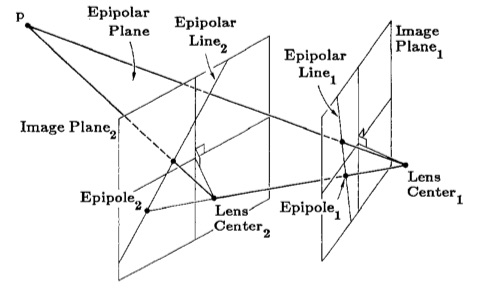
\includegraphics[width = 0.85\textwidth]{./Diagrams/epipolarline.jpg}
\caption{Stereo vision configuration, Figure taken from \cite{Bolles} p. 14}
\label{fig:epipolarline}
\end{figure}

For each point $P$ in the scene, there is a plane, called the \textit{epipolar plane}, that passes through the point and the line joining the two lens centers. The set of all epipolar planes is the \textit{pencil} of planes passing through the line joining the lens centers. Each epipolar plane intersects the two image planes along \textit{epipolar lines}. All the points in an epipolar plane are projected onto one epipolar line in the first image and onto the corresponding epipolar line in the second image. 

\bigskip

This lines are important for stereo processing since they reduce the search required to find matching points from two dimensions to one; thus, to find a match for a point along an epipolar line in one image, is just necessary to search along the corresponding epipolar line in the second image; this is equivalent to the already mentioned \textit{epipolar constraint} for a sequence of two images. Finally an \textit{epipole} is the intersection of an image plane with the line joining the lens centers.

\bigskip

The epipolar constraint can be generalized for sequences of more than two images when the camera is moving in straight line and all the lenses centers are collinear, so all pairs of camera positions produce the same pencil of epipolar planes, then straight line motion of camera defines a partition of the scene into a set of planes. If the lenses centers are not in a line, the epipolar planes passing through a scene point differe in between cameras so the one-dimensional search feature will not be possible. 

\bigskip 

Since the point of an epipolar plane are projected onto one line in each image, all the info about them is contained in that sequence of lines, the image constructed from this sequence of line is called \textit{epipolar plane image}(EPI) and contains all the information about the epipolar plane (check Figure~\ref{fig:EPI-dices})

\begin{figure}[h!]
\centering
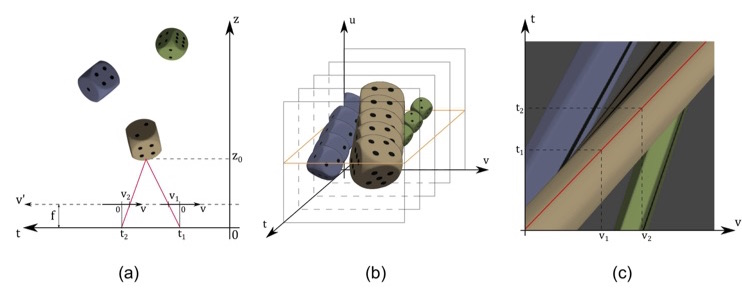
\includegraphics[width = 0.95\textwidth]{./Diagrams/EPI-dices.jpg}
\caption{Epipolar plane image (EPI) formation, (a) Capturing setup, (b) Stack of captured images, (c) Example of EPI\@. Figure taken from \cite{LF-Shearlets} page 2}
\label{fig:EPI-dices}
\end{figure}

If one has the EPI of a sufficiently dense sequence, one can estimate then the depth of each point of the scene with the slope of the lines in the EPI using Equation~\ref{eq:C1S4E2} and obtain the depth map. 

\section{Physical and computational setup for sparse acquisition of epipolar plane}
\label{sec:Sparse-acquisition}

One of the downsides on the references in this topic that we found out was the lack of detailed explanation of the followed pipeline that the group or researcher in question used to take and process the set of images of a scene, to go from a sequence of raw pictures to the epipolar plane images of the sequence; in most of the papers and books one gets a black box of expensive privative computer vision software used to detect and track pictures in the sequence; in some papers is also not clear the whole reconstruction procedure in the sense that they just present the algorithm but not the implementation code which makes impossible to reproduce and improve their implementation.

\bigskip

In this thesis we are trying to make every single detail clear in order to give the reader the tools to try themselves each step of the acquisition/processing/reconstruction technique and if possible improve it. 

\subsection{Physical setup and sampling rate}
\label{sec:phys_setup_sampling_rate}

We already saw that there are a plenty of techniques on acquire the light field of a scene, and we will use the approach of multiple views of a moving camera proposed by Bolles et al.\ 

\bigskip 

By lack of equipment we did not take the images but used the datasets provided by the research group of Professor Markus Gross in the Disney Research Center at Zurich used for their publications \cite{ChangilPhD}, \cite{PointCloud}, \cite{SceneRec} and \cite{StructMot}, all of them about scene reconstruction, outlier removal and motion flow applied to new filming techniques. One can find the datasets in their webpage \url{https://www.disneyresearch.com/project/lightfields/} with detailed description of their setting. 

\bigskip

They provide five different datasets that are made of sequence of images named after the objects that appear in the scene: Mansion, Church, Couch, Bikes and Statue; this datasets have been widely used by the community (see \cite{LF-Shearlets}). In all the cases they used a digital SLR camera translated motorized linear stage to capture the multiple views (with the camera facing perpendicularly with respect of the stage). One can observe in Figure~\ref{fig:setting} the used stage and camera.

\begin{figure}[h!]
\centering
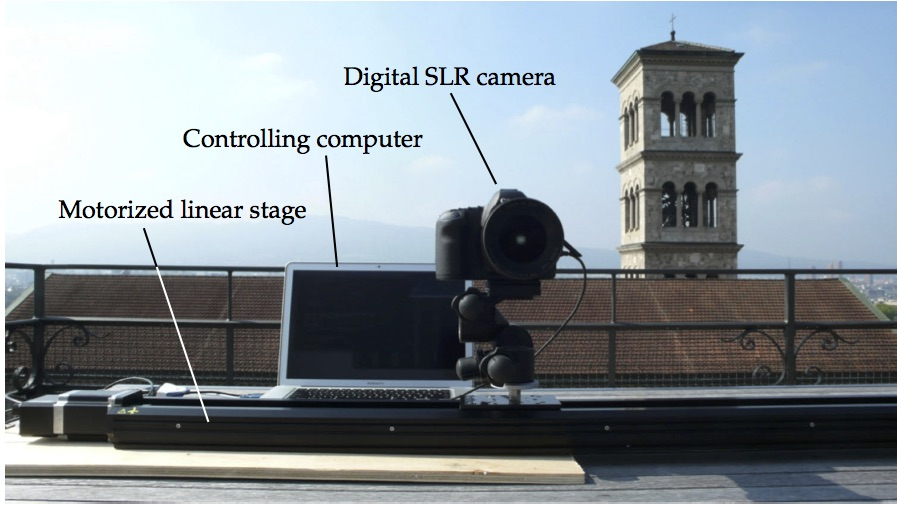
\includegraphics[width = 0.93 \textwidth]{./Diagrams/setting.jpg}
\caption{Acquisition setup with a digital SLR camera translated by a motorized linear stage, both controlled remotely from a computer. Figure taken from \cite{ChangilPhD} p.27}
\label{fig:setting}
\end{figure}

\bigskip

The reconstruction of the light field in a scene has some restrictions in the sampling rate, it is clear that successive views that are too separate from each other will make the task more difficult if not impossible. Recalling Equation~\ref{eq:C1S4E1} we have that 
$$
\Delta U = \Delta X\frac{h}{D}
$$

where $\Delta X$ is the distance traveled by the camera between succesive views, $\Delta U$ is the distance the feature moved in the image plane, $h$ the focal distance (distance between the lens center and the image plane) and $D$ the distance between the stage where the camera is moving and the feature point. 

\bigskip

Following the idea of Vagharshakyan et al. \cite{LF-Shearlets}, by assuming a horizontal sampling rate $\Delta U$ satisfying the Nyquist sampling criterion for scene's highest texture frequency, i.e.\ the sampling frequency is at least the double of the scene's highest texture frequency, one can relate the required camera motion step (sampling) with the scene depth. For given $D_{min}$ the sampling rate $\Delta X$ should be such that 

\begin{equation}
\label{eq:C2S5E4}
\Delta X \leq \frac{D_{min}}{h}\Delta U
\end{equation}

in order to ensure maximum 1 pixel disparity between nearby views, which will avoid aliasing and other artifacts. Vagharshakyan et al.\ also proved that by selecting the equality for $\Delta X$ in Equation~\ref{eq:C2S5E4}, one maximizes the baseband support, which helps in designing reconstruction filters; in particular, simple separable filters like linear interpolators can be used. The problem in this thesis is the reconstruction densely sampled EPIs (and thus the whole LF) from their decimated and aliased verrsion produced by a higher camera step $\Delta X$ than the one in Equation~\ref{eq:C2S5E4} by using some sparse representation of the EPIs. 


\bigskip

In the case of the setting used by the group of the Disney Research Center, the images were captured by using a Canon EOS 4D Mark II DSLR camera and a Canon EF $50$mm f/$1.4$ USM lens and a Zaber T-LST1500D motorized linear stage to drive the camera to the shooting positions. The camera focal length was $50$ mm and the sensor size was $36\times24$mm, PTLens was used to radially undistort the captured images, and Voodoo Camera Tracker was used to estimate the camera poses for rectifiction (is very important that the images are rectified to be able to track points); by its number of corners (features easy to track) the \textbf{Church} data set which consists in 101 pictures was the one studied in this thesis, here the camera separation is $\Delta X=10mm$ which attains the Nyquist sampling bound mentioned in Equation~\ref{eq:C2S5E4}.

\subsection{Followed pipeline}

The next diagram shows the general followed pipeline from acquisition to LF reconstruction:

\begin{center}
\begin{tikzpicture}
  [node distance=.8cm,
  start chain=going below,]
     \node[punktchain, join] (acqui) {Acquisition of rectified images sequence};
     \node[punktchain, join] (corner) {Corner detection};
     \node[punktchain, join] (tracking) {Point tracking};
     \node[punktchain, join] (paintsparse) {Initial sparse EPI painting};
     \node[punktchain, join, ] (sparserec) {Sparse EPI reconstrution};
\end{tikzpicture}
\end{center}

The last part of diagram can be represented diagramatically by Figure~\ref{fig:EPI_rec}

\begin{figure}[h!]
\centering
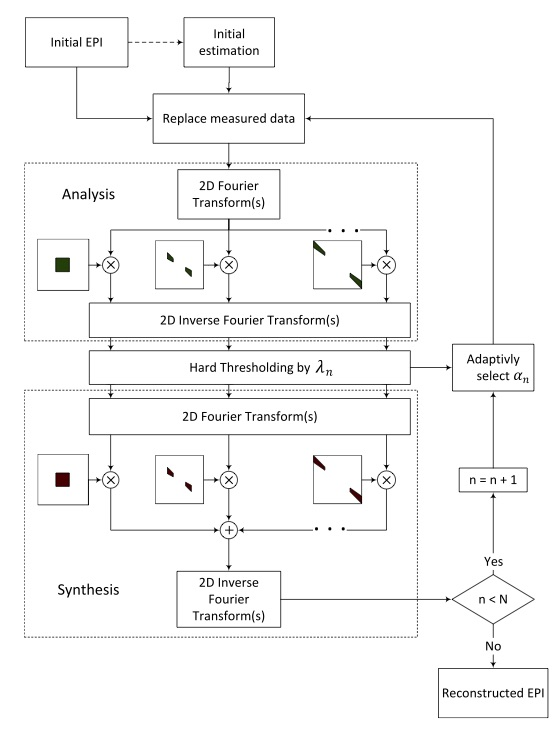
\includegraphics[width = 0.65\textwidth]{./Diagrams/Sparse_rec_diagram.jpg}
\caption{Diagram of sparse EPI reconstruction algorithm, Figure taken from \cite{LF-Shearlets} p. 7}
\label{fig:EPI_rec}
\end{figure}

The first step in the pipeline (Acquisition of rectified images sequence) was already explained in Subsection~\ref{sec:Sparse-acquisition}; the three middle steps (corner detection, point tracking and initial sparse EPI painting) will be explained in the last subsections of this chapter. Finally the last step (sparse EPI reconstructin) will be described in detail in Chapter~\ref{chap:Inpainting_sparse}.

\subsection{Geometric construction of epipolar lines}

To have closer in mind, in stereo vision when we have two different points of views of a scene (that can be interpreted as two different cameras pointing to the same scene) a line that passes through the lens center of one camera maps to a point P in the image plane and to a line in the image plane of the other camera, this line is called epipolar line, see Figure~\ref{epipolar_line}

\begin{figure}[h!]
\centering
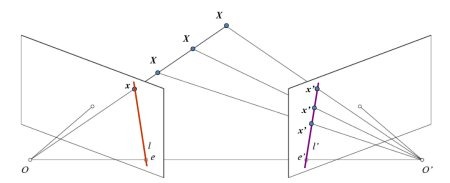
\includegraphics[width = 1\textwidth]{./Diagrams/epipolar_line.jpg}
\caption{Epipolar line correspondent to a scene point $X$. Figure taken from \url{http://opencv-python-tutroals.readthedocs.io/en/latest/py_tutorials/py_calib3d/py_epipolar_geometry/py_epipolar_geometry.html}}
\label{epipolar_line}
\end{figure}

As we mentioned, every point on the line $OX$ projects to the same point on the left image plane, this implies that just with one image we cannot triangulate the 3D point on the scene. If the points $x$ and $x'$ (corresponding to the same scene point) on the two image planes are known the proyection lines ($Ox$ and $O'x'$) most intersect exactly at X, so the coordinates of points $X$ on the scene can be calculated from the coordinates of the two image points; this means that with two perspectives is possible to triangulate 3D points. The epipolar geometry is based in this result. 

\bigskip

Let $l'$ be the epipolar line in the right image plane correspondint to $X$, this is also the projection of the line $OX$ on this image plane, by epipolar constraint to find the matching point in the right image one needs just to search in the epipolar line correspondent to $X$, this allows us to have a better performance and accuracy in feature tracking algorithms. The plane $XOO'$ is called \textit{epoipolar plane}. All the epipolar lines at each image intersect in one point called the epipole (in the Figure~\ref{epipolar_line} the epipoles correspond to the points $e$ and $e'$) and every epipolar plane pass throught the epipoles; one can also find the epipoles with the intersections of the line that joins the lens centers $O$ and $O'$ and the image planes.

\bigskip

To be able to construct algorithmically the epipolar lines we used the method implemented in the famous computer vision toolbox OpenCV (\url{http://opencv.org/}), where one can use the concepts of \textbf{Fundamental Matrix (F)} and \textbf{Essential Matrox (E)}; this matrices include all the realtive spatial information of one of the image planes with respect to the other (rotation and translation), see Figure~\ref{fig:essential_matrix.jpg}

\begin{figure}[h!]
\centering
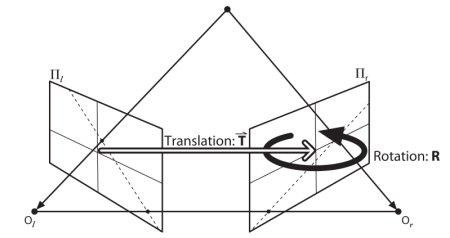
\includegraphics[width = 0.9\textwidth]{./Diagrams/essential_matrix.jpg}
\caption{Essential Matrix. Figure taken from \url{http://opencv-python-tutroals.readthedocs.io/en/latest/py_tutorials/py_calib3d/py_epipolar_geometry/py_epipolar_geometry.html}}
\label{fig:essential_matrix.jpg}
\end{figure}

Lets define and construct precisely both matrices:
\begin{itemize}
\item \textbf{Essential Matrix (E):} It contains the information about rotation and translation of the image plane, which decribes the location of the second camera relative to the first in global coordinates (i.e.\ euclidean spatial coordinates of the 3D scene). To construct it lets pick one coordinate system to work in and do our calculations from there, for instance lets coose our coordinates centered on $O_l$ (left camera's center), in this coordinates the location of the observed point $P$ is $P_l$ and the origin of the other camera is at $T$. The location of $P$ as seen by the right camera is $P_r$ in our coordinate system, where 

\begin{equation}
\label{eq:C2S5E5}
P_r=R(P_l-R)
\end{equation}

with $R$ the associated rotation matrix, to relate this we need to introduce the epipolar plane. The equation of a plane which passes trough a point $a$ with normal vector $n$ is $(x-a)\cdot n=0$, in this case the coordinates of the point $P_l$ which is in the epipolar plane will be 
\begin{equation}
\label{eq:C2S5E6}
(P_l-T)^{\intercal}(T\times P_l)=0
\end{equation}

combining Eq.~\ref{eq:C2S5E5} and Eq.~\ref{eq:C2S5E6} we obtain then that $(P_l-T)=R^{-1}P_r$, but rotation matrix are orthogonal so $R^{\intercal}=R^{-1}$ then $(R^{\intercal}P_r)^{\intercal}(T\times P_l)=0$, one can define then the matrix $S$ such that $T\times P_l=SP_l$ so 
$$
S=
\left(\begin{matrix}
0 & -T_z & T_y \\
T_z & 0 & -T_x \\
-T_y & T_x & 0
\end{matrix}\right)
$$

this imples that $(P_r)^{\intercal}RSP_l=0$. One defines $E=(P_r)^{\intercal}EP_l$ (where $E$ is the essential matrix), now to get back to global coordinates, one uses the projection equations $p_l=f_lP_l/Z_l$ and $p_r=f_rP_r/Z_r$; divinding them by $Z_l>_r/f_lf_r$ one obtains the equation for the epipolar line:
\begin{equation}
\label{eq:C2S5E7}
p_r^{\intercal}Ep_l=0
\end{equation}
since the essential matrix $E$ is a rank deficient matrix (i.e.\ if $E$ is of size $n\times n$ there are fewer $n$ nonzero eigenvalues) the Equation~\ref{eq:C2S5E7} is the equation for a line, even though we are interested in camera coordinates (pixel coordinates) and $E$ does not relates them, rather relates global coordinates, even though one can us $E$ to construct the fundamentla matrix $F$ that will do the work.

\item \textbf{Fundamental Matrix (F):} It contains the same information as $E$ in addition to information about the intrinsic of the cameras (pixel coordinates). If $p$ is a point and $M$ is the camera intrinsic matrix (which projects the image to the pixels), then $q=Mp$ is a point in the camera's coordinates, using this and the Equation~\ref{eq:C2S5E7} one has 
\begin{equation}
\label{eq:C2S5E8}
q_r^{\intercal}(M_r^{-1})^{\intercal}E M_l^{-1}q_l=0
\end{equation}
so one defines the fundamental matrix $F$ as $F=(M_r^{-1})^{\intercal}EM_l^{-1}$ so that $q_r^{\intercal}Fq_l=0$, then $F$ is just like $E$ but $F$ operating in the image pixel coordinates rather than in the physical coordinates.
\end{itemize}
it is clear that finding the epipolar lines does not require complicated mathematical concepts just linear algebra and classical geometry, for a more detailed explanation of the fundamental and essential matrices and its implementation in OpenCV we recommend the chapter 12 of \cite{LearnOpenCV} which is strongly based on the more theoretical book "Multiple View Geometry in Computer Vision" by R. Hartley and A. Zisserman \cite{MultipleView}. We are assuming here that we have a form to find matching points in between the images, but this is in our experience the hardest task on the EPI construction, and there are different ways to tackle which we will explain in the next subsection. 

\subsection{Tracking point algorithms}

Tracking a point in a sequence of images of the same scene is a very common task in computer vision; it can be applied to analyse motion flow in a video in order to predict position of an object in future frames. The task consists mainly in two part: first you need to detect feature points that are easy to track (e.g.\ corners) and second you need to follow them in the different frames. In this subsection we will present first some feature detection algorithms that are used commonly in motion flow tracking with the advantages and disadvantages of each one. 

\begin{itemize}
\item \textbf{SIFT (Scale Invariant Feature Transform):} As its name suggests it SIFT is a feature detector that is scale invariant. In the universe of computer vision related algorithms there exist plenty of imagefeature detection algorithms; some of them are corner detectors which are rotation invariant (e.g. Harris and Shi Tomasi), i.e.\ even if the image is rotated we can find the same corners; this makes a lot of sense sicne corners remain corners even if the image is rotated, but they are not necessarily scaling invariant, for example a corner in a small image within a small window is flat when is zoom in with the same window, see Figure~\ref{fig:ScalingCorner}

\begin{figure}[h!]
\centering
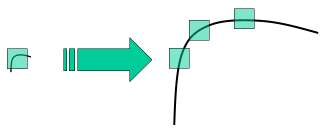
\includegraphics[width=0.7\textwidth]{./Diagrams/ScalingCorner.jpg}
\caption{Scaling a corner with constant window size does not output a corner. Figure taken from \url{http://docs.opencv.org/trunk/da/df5/tutorial_py_sift_intro.html}}
\label{fig:ScalingCorner}
\end{figure}

In 2004, D. Lowe of University of British Columbia published the paper "Distintive Image Features from Scale-Invariant Key Points" \cite{SIFT} where he presented this scaling-invariant feature detector that is known as the first of its kind and state of the art (OpenCV contains an implementation of the algorithm just in the developers version of the API). 

\bigskip

The brad idea of the algorithm is as follows: From the Figure~\ref{fig:ScalingCorner} is obvious that to detect windows with different scale. It behaves correctly with small corners, but to detect large corners we need larger windows. For this, scale-space filtering is used; Laplacian of Gaussian (refering to the famous blob detector spatial filter nicely explained in \cite{MVision}) is found for the image with various standard derivation $\sigma$ (which controls the scales); this acts as a blob detector for blobs of different sizes. One finds the local maxima accross the space and scale which give us a list of $(x,y,\sigma)$ values (see Figure~\ref{fig:dif_sizes_corners}) which means there is a potential key point $(x,y)$ at scale $\sigma$

\begin{figure}[h!]
\centering
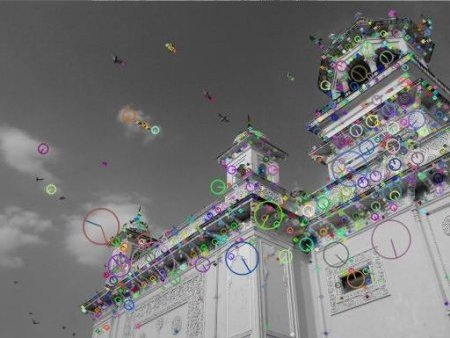
\includegraphics[width = 0.8\textwidth]{./Diagrams/dif_sizes_corners.jpg}
\caption{OpenCV implementation of SIFT algorithm that detects corners of different sizes. Figure taken from \url{http://docs.opencv.org/trunk/da/df5/tutorial_py_sift_intro.html}}
\label{fig:dif_sizes_corners}
\end{figure}

To draw the epipolar lines of a pair of images we can use SIFT as the feature points matching algorithm but is not very useful when trying to track the same points in a lot of successive images for two main reasons; first is very costly computationally since it needs to detect corners several times for different sizes and second, in the practice when we tried to implement it with OpenCV it was not mantaining the order of the corners so when we have too many corners there was not a straight-forward way to keep track along the sequence of pictures.

\item \textbf{Harris Corner Detector:} This corner detector was introduced by Chris Harry and Mike Stephens in the 1998 paper "A combined corner and edge detector" \cite{HarrisCorner}, and their idea was very simple. This algorithm basically finds the difference in intensity for a displacement of $(u,v)$ in all directions. This is expressed as bellow:

\begin{equation}
\label{eq:C2S4E9}
E(u,v)=\sum_{x,y}w(x,y)(I(x+u,y+v)-I(x,y))^2
\end{equation}

where $w$ is a windows function (e.g.\ rectangular or gaussian), and $I(x,y)$ is the intensity of the image at the point $(x,y)$. For corner detection one has to maximize the functional $E(u,v)$, applying Taylor expansion one gets the equation 
$$
E(u,v)\approx
 \left(
\begin{matrix}
u &  v
\end{matrix}
\right)
M
\left( 
\begin{matrix}
u\\
v
\end{matrix}
\right)
$$
where
$$
M = \sum_{x,y}w(x,y)
\left(\begin{matrix}
I_xI_x & I_xI_y \\
I_xI_y & I_yI_y
\end{matrix}
\right)
$$
where $I_x$ and $I_y$ are directional derivatives of the intensity. The main part comes when after this they created a score, this scores will indicate if a window can contain a corener or no and is given by the following relation
\begin{equation}
\label{eq:C2S4E10}
R=det(M)-K(\tr{(M)})^2=\lambda_1\lambda_2-K(\lambda_1+\lambda_2)^2
\end{equation}
where $\lambda_1$ and $\lambda_2$ are the eigenvalues of $M$. The criterion with the score has the next cases:
\begin{enumerate}
\item If $|R|$ is small, i.e.\ $\lambda_1,\lambda_2$ are small, the region is flat.
\item If $R<0$, i.e.\ $\lambda_1\gg\lambda_2$ or viceversa, the region is an edge.
\item If $R$ is large, $\lambda_1$ and $\lambda_2$ are large and $\lambda_1\sim\lambda_2$, then region is a corner. 
\end{enumerate}
for a graphical representation of this conditions see Figure~\ref{fig:harris_region}.

\begin{figure}[h!]
\centering
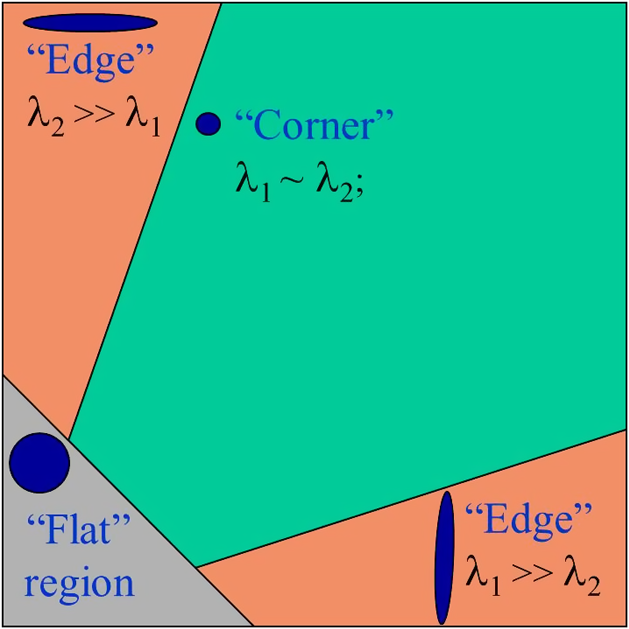
\includegraphics[width = 0.5\textwidth]{./Diagrams/harris_region.png}
\caption{Diagrama representing the criterion of corner detection for Harris detector, the axis $x$ represents $\lambda_1$ and axis $y$ represents $\lambda_2$}
\label{fig:harris_region}
\end{figure}

OpenCV offers a faithful implementation of Harris Corner Detector, but we rather used a modification of this algorithm that works better, the so called Shi-Tomasi Corner Detector.

\item \textbf{Shi-Tomasi corner detector:} After Harris and Stephens proposed their corner detector in 1994 J. Shi and C. Tomasi proposed a variation on their paper "Good Features to Track" \cite{ShiTomasi} which shows better results compared with Harris work. 

\bigskip

Shi-Tomasi changes the scoring function that gave criteria for corner detection in Harris (see Equation~\ref{eq:C2S4E10}) to the form
\begin{equation}
\label{eq:C2S4E11}
R = \min (\lambda_1,\lambda_2)
\end{equation}
as in the case of the Harris Corner Detector, if $|R|$ is greater than a threshold value $\lambda_{\min}$, it is considered as a corner. The $\lambda_1\text{vs.}\lambda_2$ space will now look as in Figure~\ref{fig:shitomasi_space}

\begin{figure}[h!]
\centering
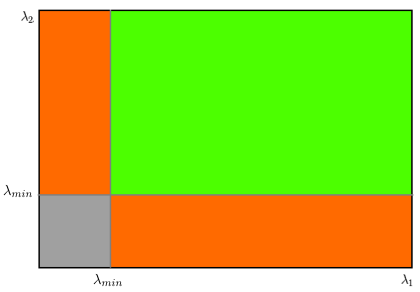
\includegraphics[width=0.7\textwidth]{./Diagrams/shitomasi_space.png}
\caption{$\lambda_1\text{vs.}\lambda_2$ space for Shi-Tomasi corner detector, as in Harris detector's case, the upper right area corresponds to corners, the upper left and lower right correspond to edges}
\label{fig:shitomasi_space}
\end{figure}

There is also an straight forward implementation of this algorithm on OpenCV, we used this algorithm to find the $N$ strongest corners and then trakc them with Lucas-Kanade algorithm. Even the Shi-Tomasi corner detector is rotation invariant since the trace and the determinant of the matrix $M$ are rotation invariant they are not scaling invariant like the SIFT algorithm which is slower than the former. In the case of the sequence that we are working with the images were taken very close to each other so the scale of the features wont change significantly. 
\end{itemize}

We already explained the different options for feature detection algorithms and that the option picked was the Shi-Tomasi corner detector to track the strong corners obtained by the Shi-Tomasi algorithm we used the Lucas-Kanade method explained as follows:
\begin{itemize}
\item \textbf{Lucas-Kanade method:} We would like to associate a movement vector $(u,v)$ to every such "interesting pixel" (stron corner point) in the scene obtained by comparing two successive images with the next two assumptions:
\begin{enumerate}
\item The two images are separated by a small increment $\Delta t$, such that the objects have not displaces significantly (the algorithm works best with slow moving objects). 
\item The images depict a natural scene containing textured objects exhibiting shades of gray (different intensity levels) which change smoothly.
\item The pixel intensity of an object does not change in consecutive frames.
\item Neighbouring pixels have similar motion.
\end{enumerate}
With this assumptions consider a piel in $(x,y)$ at time $t$ with intensity $I(x,y,t)$, it moves by distance $(dx,dy)$ in next frame taken after $dt$ time. Since those pixels are the same and intensity does not change we can say 
$$
I(x,y,t)=I(x+dx,y+dy,t+dt)
$$
Expanding with Taylor the right hand side we obtain the following equation
\begin{equation}
\label{eq:C2S5E12}
I_xu+I_yv+I_t=0
\end{equation}
where 
$$
\begin{aligned}
I_x &= \frac{\partial I}{\partial x}&;
I_y &= \frac{\partial I}{\partial y}\\
I_t &= \frac{\partial I}{\partial t}\\
u &= \frac{\partial x}{\partial t}&;
v &= \frac{\partial y}{\partial t}
\end{aligned}
$$
The Equation~\ref{eq:C2S5E12} is known as the \textbf{"Optical Flow Equation"}.Computing the gradient of the intensity we obtain $(I_x,I_y,I_t)$, and we aim to know the flow by solving the equation for $(u,v)$. In 1981, Bruce D. Lucas and Takeo Kanade proposed a method to solve this in their paper "An iterative image registration technique with an application to stereo vision" \cite{LucasKanade}; the made the assumptions that we already mentioned before. 

\bigskip

By assumption neighbouring pixels have similar motion, lets take a $3\times 3$ patch around the point (in our case corner), then all the nine points of the patch have the same motion. We can find $(I_x,I_y,I_t)$ for this nine points; thus the problem reduces to solve nine equations with 2 unknowns variables which is over-determined. As is explained in detail on \cite{LucasKanade} a better solution is obtained with least squares fit method. In this setting the problem has the solution
\begin{equation}
\label{eq:C2S5E13}
\left( 
\begin{matrix}
u \\
v 
\end{matrix}
\right) = 
\left(
\begin{matrix}
\sum_i I_{x_i}^2 & \sum_i I_{x_i}I_{y_i} \\
\sum_i I_{x_i}I_{y_i} & \sum_i I_{y_i}^2 
\end{matrix}
\right)^{-1}
\left(
\begin{matrix}
-\sum_i I_{x_i}I_{t_i}\\
-\sum_i I_{y_i}I_{t_i}
\end{matrix}
\right)
\end{equation}
obtaining with this the vector flow of the features in the scene. By its simplicity we used the OpenCV implementation of this algorithm to track the $N$ strongest corners (found by Shi-Tomasi corner detector) in the image sequence \textbf{Church}. In the next subsection we will show explicitly how did we implemented the Lucas-Kanade methid with the Shi-Tomasi algorithm to detect and track strong corners in our dataset, including the code in python. We will also show how to paint the Epipolar plane based on the results of this procedure. 
\end{itemize}
 
\subsection{Procedure for tracking and painting the EPIs}

The maximum number of strong corners obtained by the Shi-Tomsi in the first view was 336, one can see in Figure~\ref{fig:first_frame_church} the first image of the curch and in Figure~\ref{fig:first_frame_church_points} the 336 strong corners found by the Shi-Tomasi detector; one can also see in Figure~\ref{fig:last_frame_church} the last image (number 101) of the curch and in Figure~\ref{fig:last_frame_church_points} the final position of the points correspondent to the tracked corners. Finally, in the Figure~\ref{fig:track_points_church} one can see the path of the corners tracked through the sequence of images in the data set. The code used to detect the $N$ strongest corners with Shi-Tomasi detector and track them through the sequence of images in the Church data set using Lucas-Kanade method is presented in Appendix~\ref{sec:Appendix_A}. Using this code the time elapsed to detect and track 336 corners along 101 pictures in the Church data set sequence was \textbf{16.36 seconds} in a Macbook PRO with OSX 10.10.5, with 8GB memory, 2.7 GHz Intel Core i5 processor and Graphic Card Intel Iris Graphics 6100 1536 MB. 

\begin{figure}[h!]
\centering
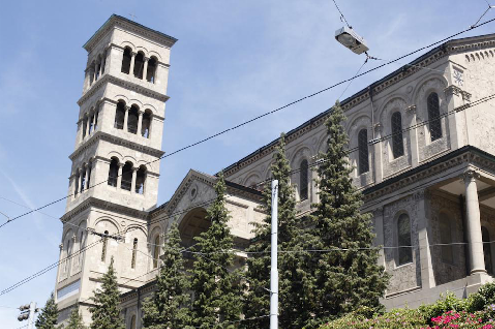
\includegraphics[width=1 \textwidth]{./Diagrams/first_frame_church.png}
\caption{First image of the church data set}
\label{fig:first_frame_church}
\end{figure}

\begin{figure}[h!]
\centering
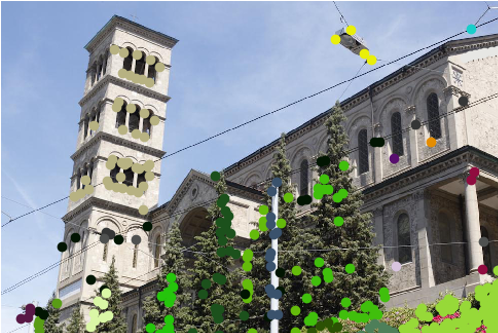
\includegraphics[width=1\textwidth]{./Diagrams/first_frame_church_points.png}
\caption{336 corners found in the first image of the church with different colors corresponding to different features}
\label{fig:first_frame_church_points}
\end{figure}

\begin{figure}[h!]
\centering
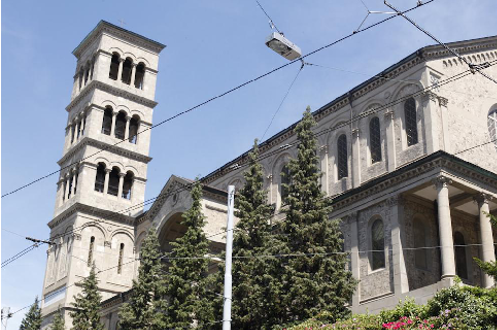
\includegraphics[width=1 \textwidth]{./Diagrams/last_frame_church.png}
\caption{Last image of the church data set}
\label{fig:last_frame_church}
\end{figure}

\begin{figure}[h!]
\centering
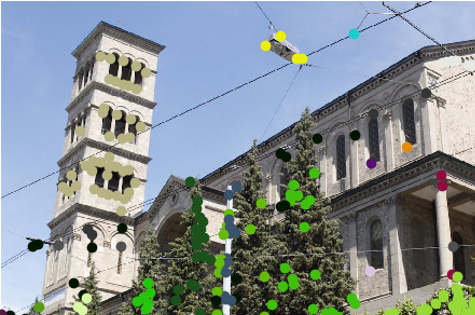
\includegraphics[width=1\textwidth]{./Diagrams/last_frame_church_points.png}
\caption{Last position of corners in the last image of the church}
\label{fig:last_frame_church_points}
\end{figure}

\begin{figure}[h!]
\centering
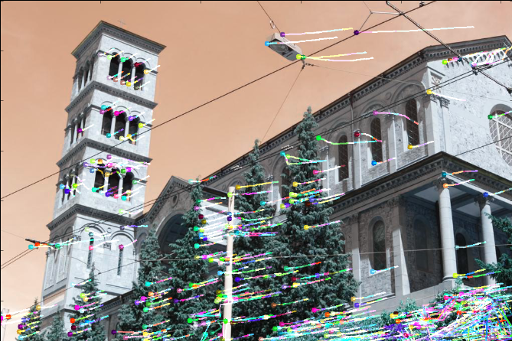
\includegraphics[width=1\textwidth]{./Diagrams/track_points_church.png}s
\caption{Path of points tracked in the image sequence of the church, one can observe that the trajectories of the features are more or less straight lines, with some nuerical and algorithmical errors that can be ignored. The image is presented in shades of gray since the Lucas-Kanade method can be implemented with good performance in shades of gray}
\label{fig:track_points_church}
\end{figure}

\bigskip

We are trying to construct the epipolar plane images correspondent to the sequence of different views of the church; for that we will follow the method that Bolles proposed in \cite{Bolles}. We will use that the points follow a straight line trajectory along the sequence due that the camera followed an straight line so each point in the first image will move in its correspondent epipolar line which will be parallel to the $x$-axis, since the camera points orthogonally with respect to the to the scene. 

\bigskip

For each strip $y_0-\epsilon \leq y \leq y_0+\epsilon$ that is parallel to the $x$-axis in the initial image we ploted for points correspondent to different features the $x$ entry (which corresponds to the $u$ entry in the two-planes 4D light field model) with respect to the time (the sequence of images).

\bigskip

Since in comparsion with the actual resolution of the pictures ($1024\text{px}\times 683\text{px}=699392\text{px}^2$) the number of corners that we could detect was very small (about 0.04\% of the total number of points) taking strips of points with constant $y=y_0$ that are very tight will not capture a lot of tracked points; the distribution of the points as one can see in Figure~\ref{fig:first_frame_church_points} is not homogeneous at all. 

\bigskip

In order to have a trustworthy light field reconstruction we took Epipolar plane images corresponding to $y$-strips with different thickness depending on the density of tracked points for the corresponding $y$, for example more tight at the bottom part of the pictures where we have a lot of tracked points due the bushes and trees and  broader at the top where there is not a lot of tracked points due the almost homogeneous sky.

\begin{figure}[h!]
\centering
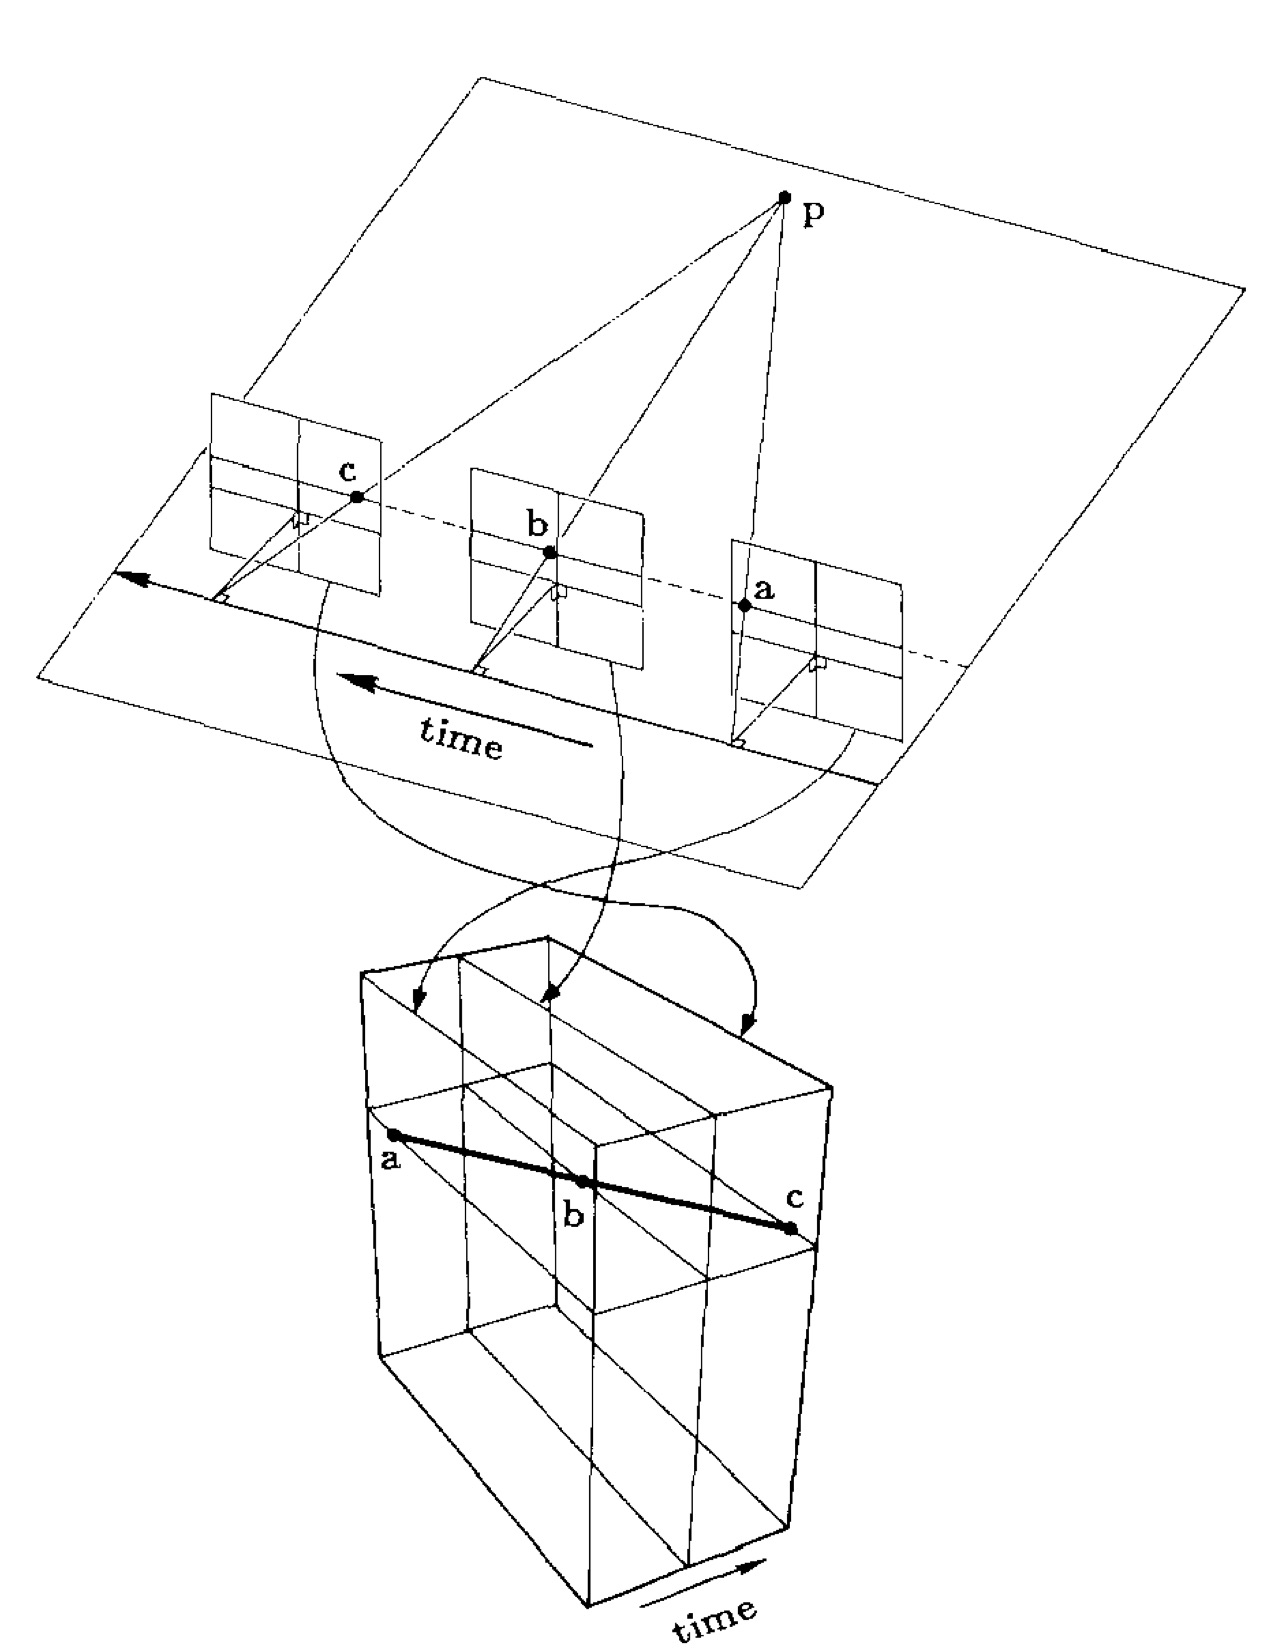
\includegraphics[width = 0.6 \textwidth]{./Diagrams/lateral_motion_epi.jpg}
\caption{Feature point tracking for lateral camera motion. Figure taken from \cite{Bolles} p. 16}
\label{lateral_motion_epi}
\end{figure}

\begin{figure}[h!]
\centering
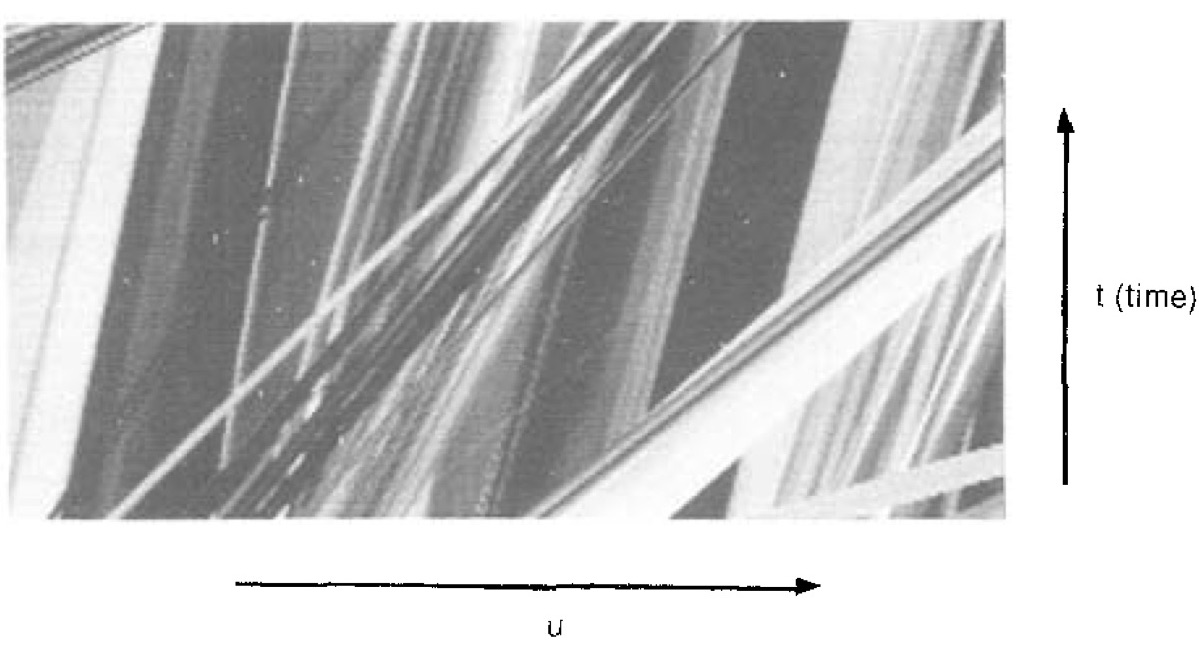
\includegraphics[width = 0.8 \textwidth]{./Diagrams/EPI_bolles.jpg}
\caption{EPI correspondent to some strip in the sequence of images, we are looking to get the EPI for the Church data set. Figure taken from \cite{Bolles} p. 17}
\label{EPI_bolles}
\end{figure}

\begin{figure}[h!]
\centering
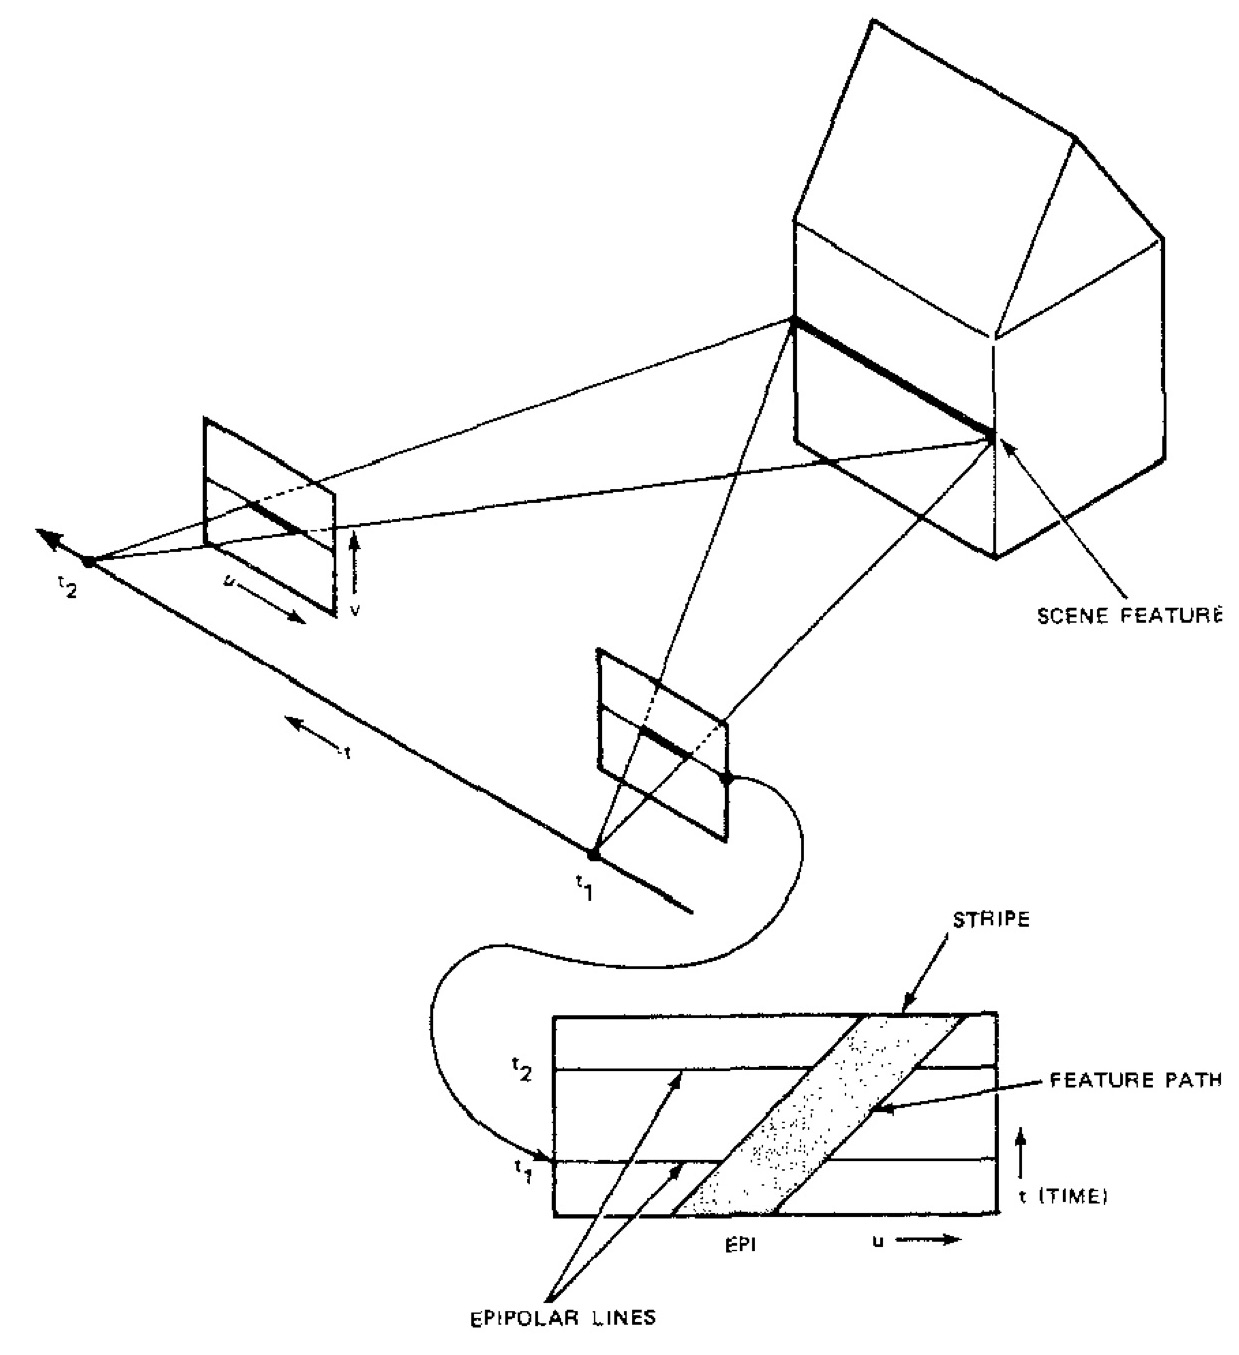
\includegraphics[width = 0.6 \textwidth]{./Diagrams/Feature_EPI_bolles.jpg}
\caption{Horizontal line of a feature (house) corresponds to a diagonal strip its correspondent EPI\@. Figure taken from \cite{Bolles} p. 17}
\label{Feature_EPI_bolles}
\end{figure}

We can see in Figure~\ref{fig:673_10_102_4_48_8_strip} a strip at the bottom of the image, centered at $y_0=673$, with width $2\epsilon=20$ that captures 48 different tracked points corresponding to 8 different features, the dense EPI associated with this strip is in Figure~\ref{fig:673_10_102_4_48_8_dense} and its sparse form obtained by measuring each 4 rows at the EPI is in Figure~\ref{fig:673_10_102_4_48_8_sparse}. We will present a deeper analysis on the sparse measure and the main results of Shearlet-based inpainting an sparse EPI and measuring the depth map which is the main topic of this thesis at Chapter~\ref{chap:Inpainting_sparse}.

\begin{figure}[h!]
\centering
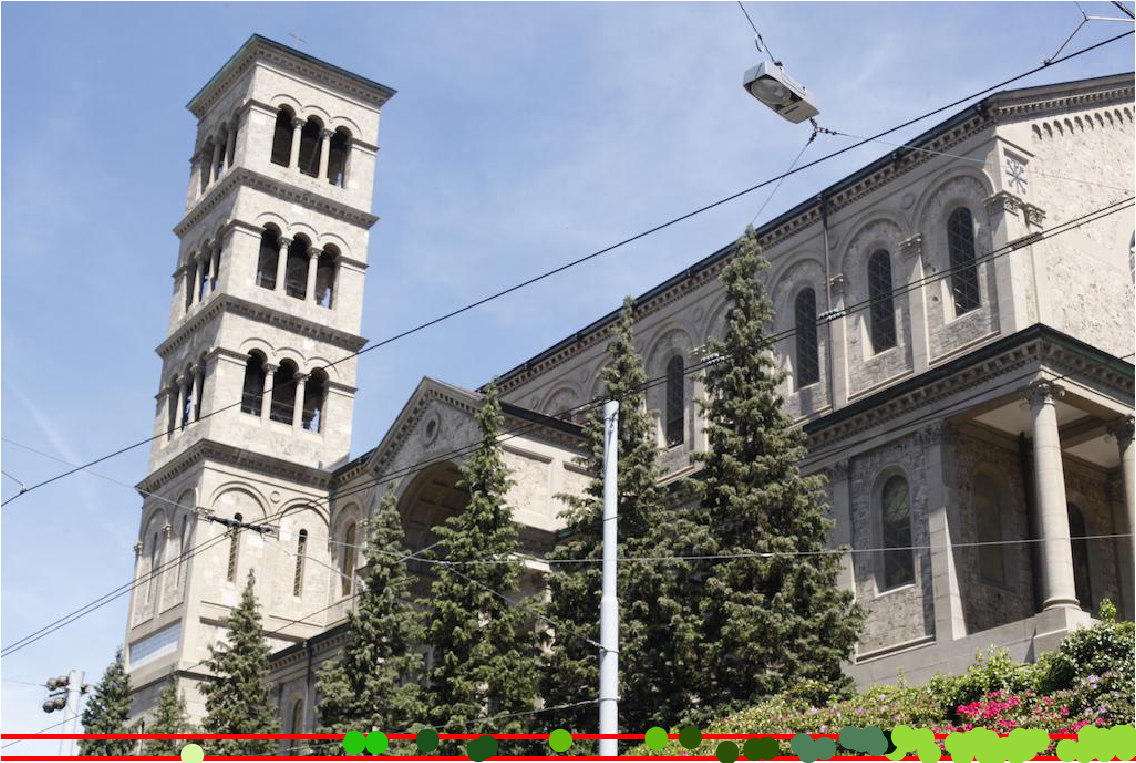
\includegraphics[width = 0.6 \textwidth]{./EPIs_Strips/EPIs/673_10_102_4_48_8_strip.png}
\caption{Tracked points on a strip centered at $y_0=673$ with width $2\epsilon=20$}
\label{fig:673_10_102_4_48_8_strip}
\end{figure}

\begin{figure}[h!]
\centering

\includegraphics[width = 0.6 \textwidth]{./EPIs_Strips/EPIs/673_10_102_4_48_8_dense.png}
\caption{Dense Epipolar plane image associated with the strip on Figure~\ref{fig:673_10_102_4_48_8_strip}, the horizontal axis is the spatial coordinate $x$ and the vertical axis is the time}
\label{fig:673_10_102_4_48_8_dense}
\end{figure}

\begin{figure}[h!]
\centering
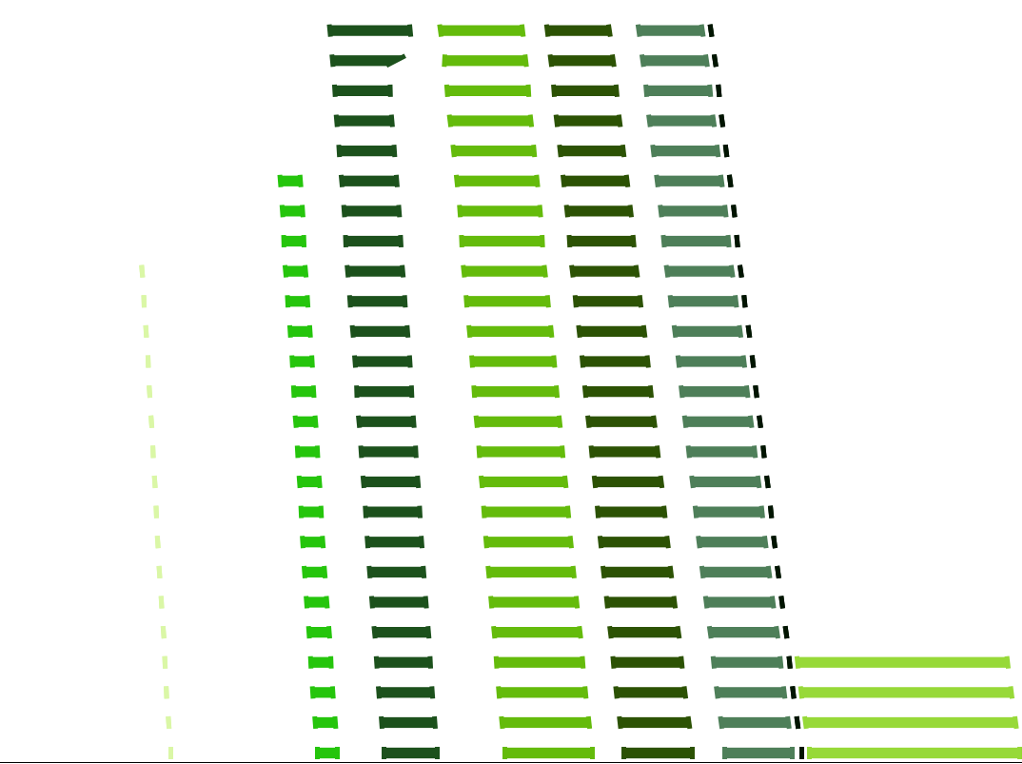
\includegraphics[width = 0.6 \textwidth]{./EPIs_Strips/EPIs/673_10_102_4_48_8_sparse.png}
\caption{Sparse Epipolar plane image associated with the strip on Figure~\ref{fig:673_10_102_4_48_8_sparse} by measuring each 4th row on Figure~\ref{fig:673_10_102_4_48_8_dense}}
\label{fig:673_10_102_4_48_8_sparse}
\end{figure}

